\chapter{SOIピクセル検出器}

\section{概要}

2005年4月よりKEK測定器開発室のプロジェクトの一つとしてSilicon On Insulator(以下SOI)技術による読み出し回路一体型ピクセル検出器の開発が開始された.SOI技術とは、回路部シリコン層と支持基板部シリコン層間に${\rm SiO_2}$の絶縁層を埋め込む技術であり、トランジスタ素子を分離することで電気的な接続を分離できるのが特徴である.読み出し回路部から検出部分へは酸化膜層BOX(Buried OXide)を貫通する金属ビアを通したセンサー電極が伸びており、センサー電極シリコンと検出部分シリコンのpn接合で検出部分に空乏層を形成する.そこに逆バイアス電圧を印加することで空乏層を広げる.空乏層へ荷電粒子が入射すれば、電子正孔対が生成され、センサー電極に移動しシグナルとして検出される.よって、どこのセンサー電極で検出されたかによって入射粒子の通過した位置を決めることができる。このSOI技術を用いることで、現在主流であるバルクCMOS技術と同じ設計ルールでも一世代進んだ特性を示す半導体を製造することが可能であり、KEKの新井康夫氏を中心にR$\&$Dが進められてきた.特に、2013年から本年度に掛けて、「3次元半導体検出器で切り拓く新たな量子イメージングの展開」として新学術領域研究に指定され、素核・宇宙・物質・生命科学の多岐に渡りSOI技術を用いた新たな量子イメージング領域の研究が行われてきた.

\begin{figure}[htbp]
			\begin{center}
				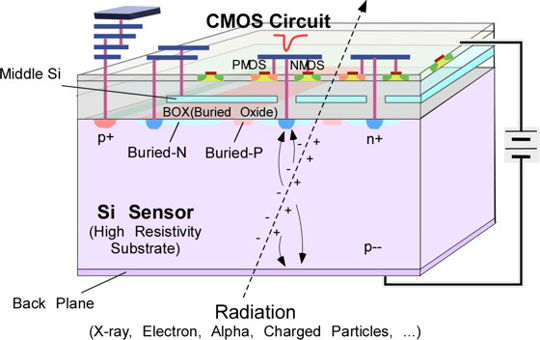
\includegraphics[width=12.0cm]{./Chapter/Chapter3/Picture/SOIPIX.png}
				\caption{SOIピクセル検出器}
				\label{fig:SOIPIX}
			\end{center}
		\end{figure}
%\begin{figure}[H]
%\begin{center}
%\includegraphics[width=120mm]{./Chapter/Chapter3/Picture/SOIピクセル検出器.png}
%\end{center}
%\caption{SOIピクセル検出器}
%\label{fig:SOI}
%\end{figure}
%\end{section}
%\clearpage

\section{SOIウエハーの特徴}
SOI技術を用いることの利点を具体的に説明する.

\section{Monolithic型検出器}
現在多くの放射線イメージセンサーには



身近にある物質の中でも金属のように電気を通すものもあれば、ガラスのように電気をほとんど通さないような物質も存在する。抵抗率の違いから、物質は大きく3種類に大別されている。
	\begin{description}
		\item[導体] 金属など電気を通しやすい物質
		\item[絶縁体] ガラスのように電気を通しにくい物質
		\item[半導体] 導体と絶縁体の中間の抵抗率を持つ物質
	\end{description}
	
	この半導体には「P型半導体」と「N型半導体」の2種類の型があり、以下それらについて説明する。
	\subsection{P型半導体とN型半導体}
		シリコンは価電子を4個持つ。純粋なシリコンの結晶中では隣り合ったシリコン原子は互いに電子を共有しあって結合している。電子は原子に束縛されている状態なので容易に動くことはできない。したがって純粋なシリコン結晶に電圧を印加しても電流はほとんど流れず、電気抵抗率は室温環境下で$10^3 \mathrm{\Omega cm}$以下である。
		
		しかし、シリコンに不純物を添加した状態で電圧を印加することによってキャリアを流すことができる。添加する物質の違いから、
		\begin{description}
			\item[P型半導体] キャリアが正孔である半導体
			\item[N型半導体] キャリアが電子である半導体
		\end{description}
		に大別することができる。P型半導体とN型半導体の概念図を図\ref{fig:Semicon_PN}に示す。
		
		P型半導体は高純度の半導体(主にシリコン)に不純物としてホウ素Bなどの3価元素をごく微量添加することによって作製できる。
		シリコンSiの価電子が4個に対して、ホウ素Bのような3価元素の価電子は3個しかないので、共有結合するのに電子が1つ足りない状況になる。
		したがって、図\ref{fig:Semicon_P}のように電子のない空席(これを「正孔」と呼ぶ)ができる。
		不純物を添加しない場合、電子は原子に束縛された状況なので動くことはできないが、ホウ素Bを添加することで正孔ができるので、結晶に電圧を印加した場合、正孔の近くにある電子は正極に引かれて正孔の方に移動する。
		そのとき、その電子がもともと存在していた場所は新たな正孔となり、その近くに存在する電子がまた移動し、正孔があたかも正(positive)の電荷を持つ粒子のように振る舞う。
		このような半導体のことを「P型半導体」と呼び、この半導体のキャリアは正(positive)の電荷を持つ「正孔」である。
		
		一方、N型半導体は高純度シリコンSiに不純物としてリンPなどの5価元素をごく微量添加することによって作製できる。
		5価元素の価電子は5個なので共有結合に電子を4個使っても電子が1つ余ってしまう。
		共有結合に使われている他の電子に比べてリン原子との束縛は弱いので、結晶に電圧を印加することによって電子は正極に引かれて動く。
		このような振る舞いを示す半導体のことを「N型半導体」と呼び、この半導体のキャリアは負(negative)の電荷を持つ「電子」である。
		%=====P型半導体とN型半導体の概念図を載せる=====%
		\begin{figure}[hbtp]
  			\begin{minipage}[b]{0.45\linewidth}
    				\centering
    				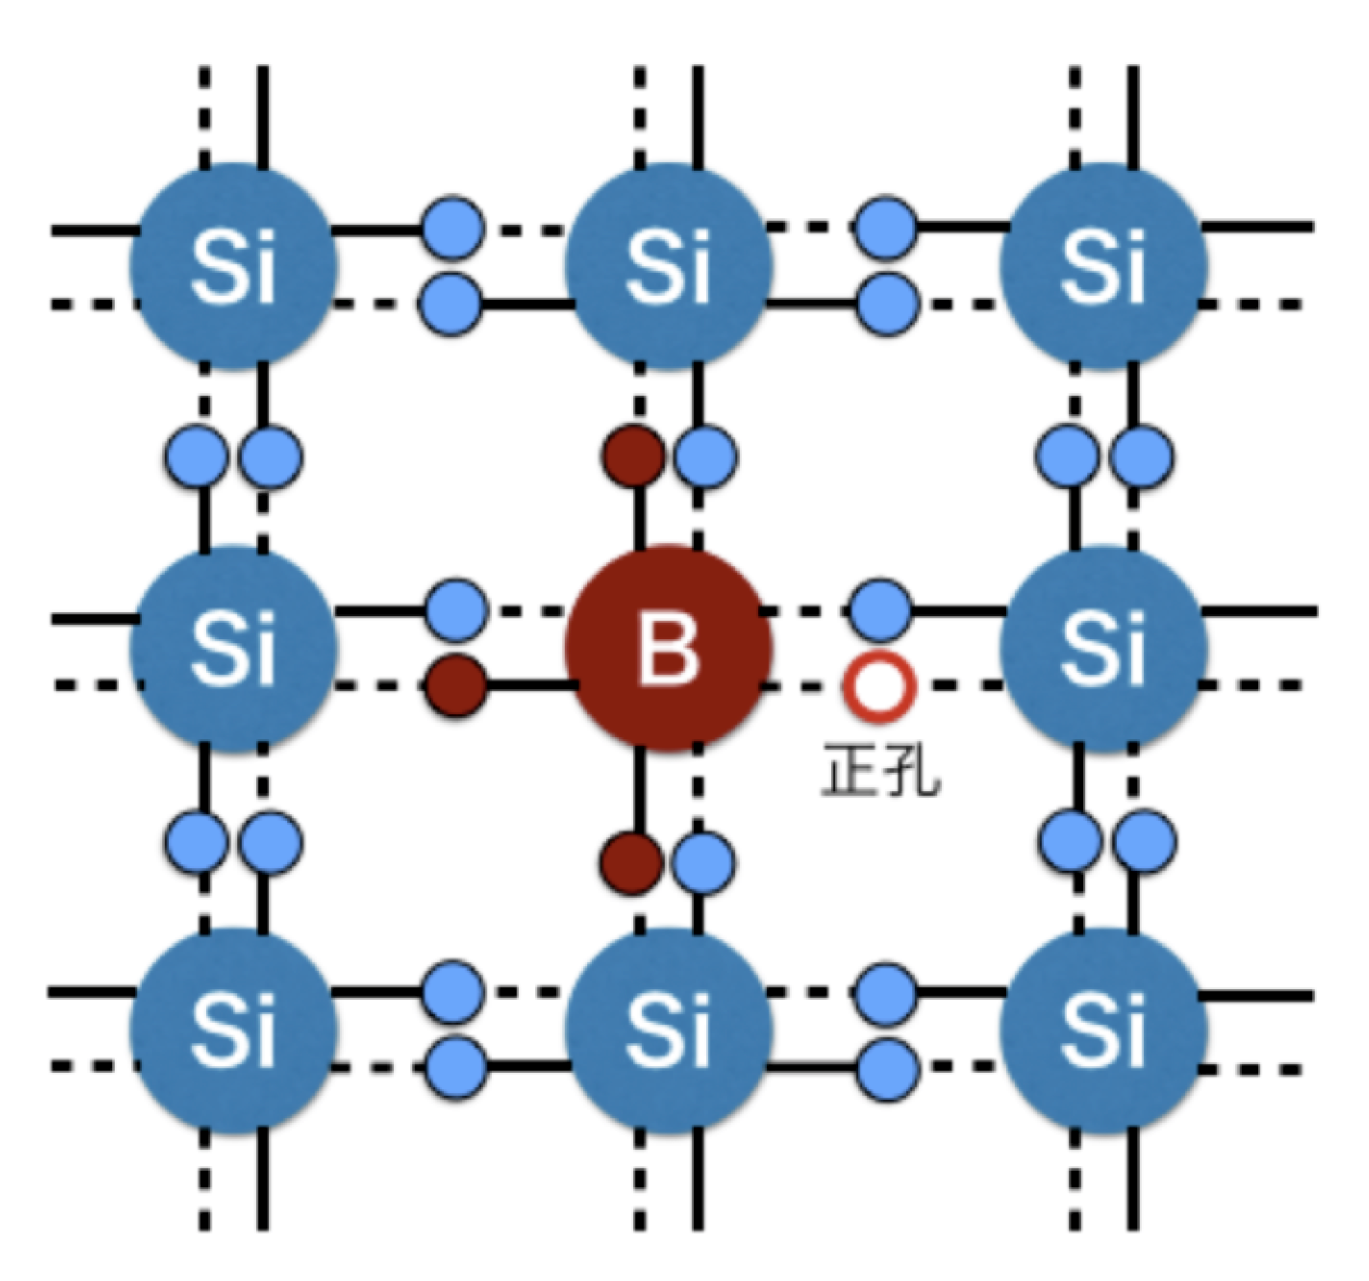
\includegraphics[keepaspectratio, scale=0.2]{./Chapter/Chapter3/Picture/Semicon_P.eps}
				\subcaption{P型半導体}
				\label{fig:Semicon_P}
  			\end{minipage}
  			\begin{minipage}[b]{0.45\linewidth}
    				\centering
    				\includegraphics[keepaspectratio, scale=0.2]{./Chapter/Chapter3/Picture/Semicon_N.eps}
    				\subcaption{N型半導体}
				\label{fig:Semicon_N}
  			\end{minipage}
 			\caption{P型半導体とN型半導体のそれぞれの概念図}
			\label{fig:Semicon_PN}
		\end{figure}
		
		半導体を用いたデバイスには2端子を基本とする「ダイオード」と3端子を基本とする「トランジスタ」がある。
		そのトランジスタには動作原理から、「電界効果トランジスタ(FET : Field Effect Transistor)」と「バイポーラトランジスタ(BJT : Bipolar Junction Semiconductor)」に大別される。
		
		我々研究グループが開発している極低温環境用前置増幅器には、この2種類のトランジスタのうちMOS(Metal Oxide Semiconductor)構造を持った電界効果トランジスタ(MOSFET)を用いることを考えている。次節は、そのMOSFETについての基礎特性について述べる。
		
\section{MOSFETの基礎}
	MOSFETには3つの端子があり、それぞれソース(S)、ゲート(G)、ドレイン(D)とよばれている。ゲート・ソース間に電圧を印加することによって、ドレイン・ソース間のキャリア密度が変化し、それによってドレイン・ソース間の電流(ドレイン電流)を制御することができる。MOSFETはドレイン・ソース間を移動するキャリアの種類によって2つの型に大別することができる。キャリアが電子の場合はN型MOSFET(NMOS)と呼ばれ、正孔の場合はP型MOSFET(PMOS)と呼ばれる。
	\subsection{MOSFETの構造}
		前述した通り、MOSFETはキャリアの種類に応じてNMOSとPMOSの2種類に大別される。図\ref{fig:MOSFET_N_structure}にNMOSの構造を示した。
		以降、NMOSについての構造について述べる。
	%=====MOSFETの構造の概念図を載せる=====%
		\begin{figure}[htbp]
			\begin{center}
				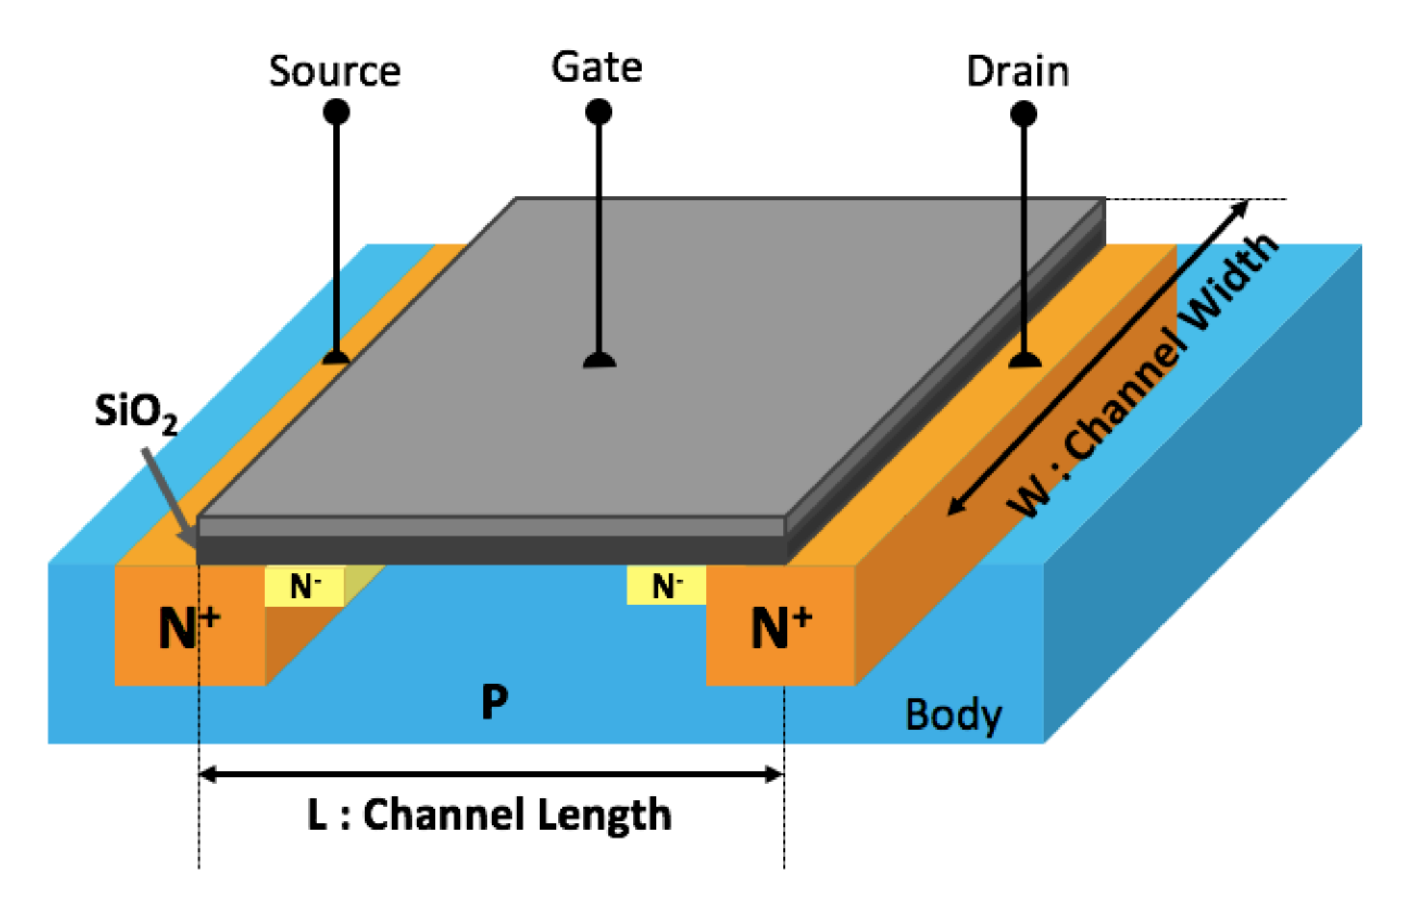
\includegraphics[width=12.0cm]{./Chapter/Chapter3/Picture/MOSFET_N_structure.eps}
				\caption{N型MOSFETの構造}
				\label{fig:MOSFET_N_structure}
			\end{center}
		\end{figure}
		P型半導体基板上に$\mathrm{N^+}$領域が2つ形成されており、それぞれソース(S : Source)、ドレイン(D : Drain)と呼ばれている。
		そして、これらの$\mathrm{N^+}$領域に挟まれたP型半導体基板の直上に酸化シリコン$\mathrm{SiO_2}$からなるゲート酸化膜が形成されており、そして更に直上に金属、あるいはポリシリコンからなるゲート電極(G : Gate)が形成されている。
		また、PN接合近傍での急激な電界勾配を回避するために、ゲートエッジ部にソースとドレインそれぞれの拡散層の不純物密度分布を緩やかにするプロセスが施されている。
		この部分を低濃度不純物ドレイン(LDD : Lightly Doped Drain)と呼ぶ。
		一方、PMOSの構造は、NMOSで用いる半導体の型を反転した構造をしており、それ以外の構造はNMOSと同じである。次節ではMOSFETの動作原理について述べる。
	\subsection{MOSFETの動作原理}
		\begin{figure}[htbp]
			\begin{center}
				\begin{tabular}{c}
					\begin{minipage}{0.33\hsize}
						\begin{center}
							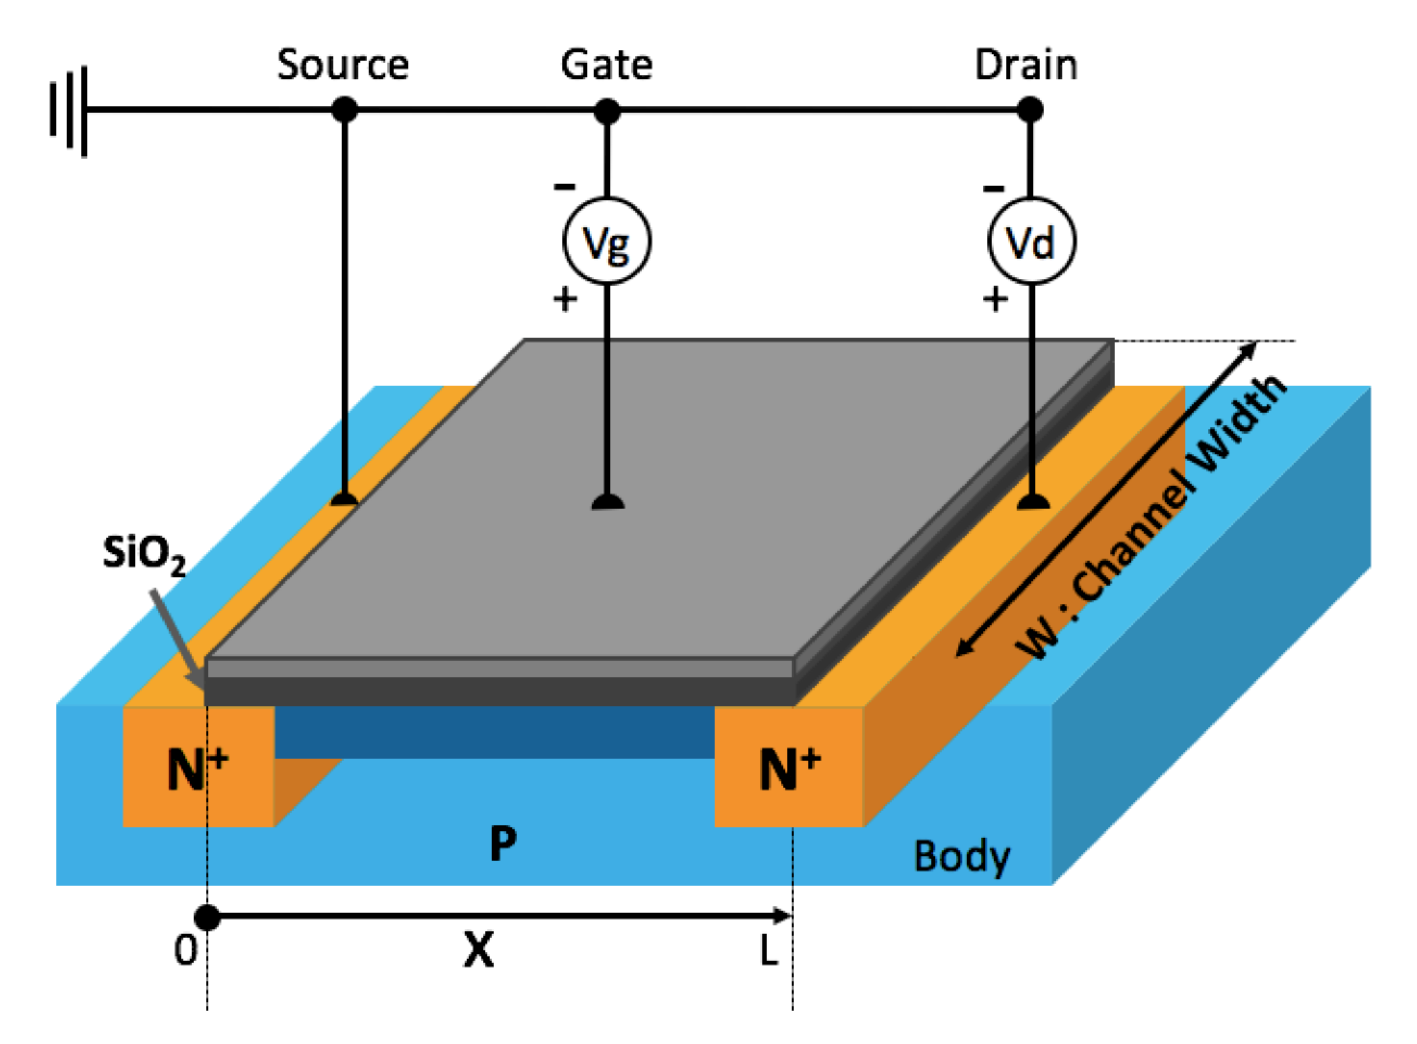
\includegraphics[clip, width=4.5cm]{./Chapter/Chapter3/Picture/MOSFET_accumulation.eps}
							\hspace{1.6cm} [1]蓄積領域
						\end{center}
					\end{minipage}
					\begin{minipage}{0.33\hsize}
						\begin{center}
							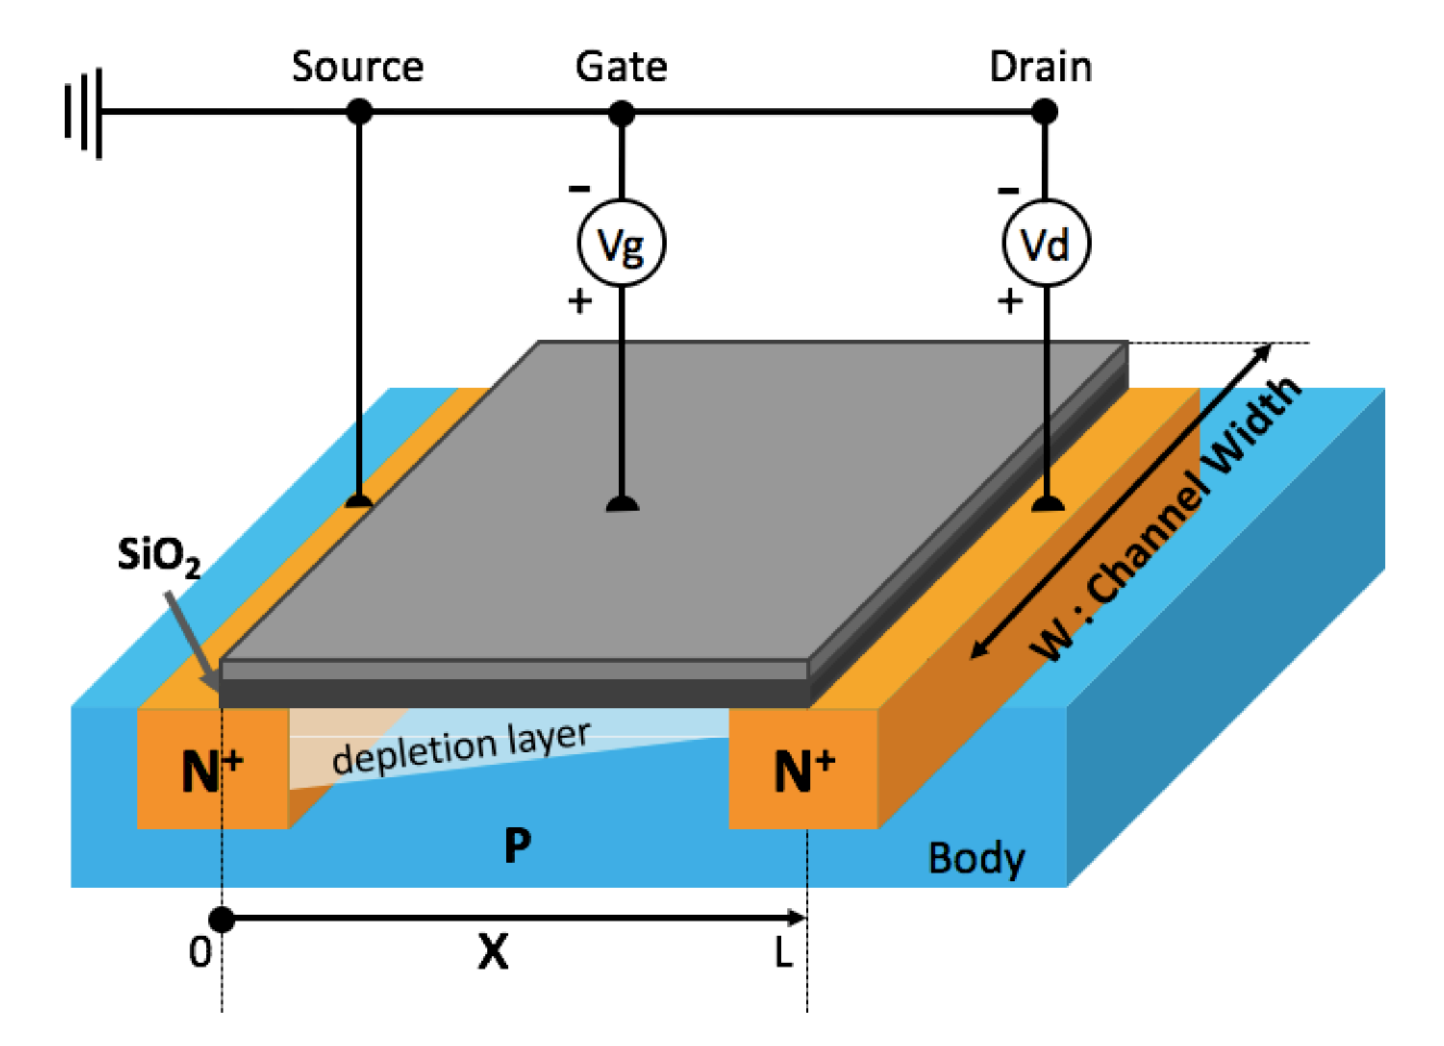
\includegraphics[clip, width=4.5cm]{./Chapter/Chapter3/Picture/MOSFET_depletion.eps}
							\hspace{1.6cm} [2]空乏領域
						\end{center}
					\end{minipage}
					\begin{minipage}{0.33\hsize}
						\begin{center}
							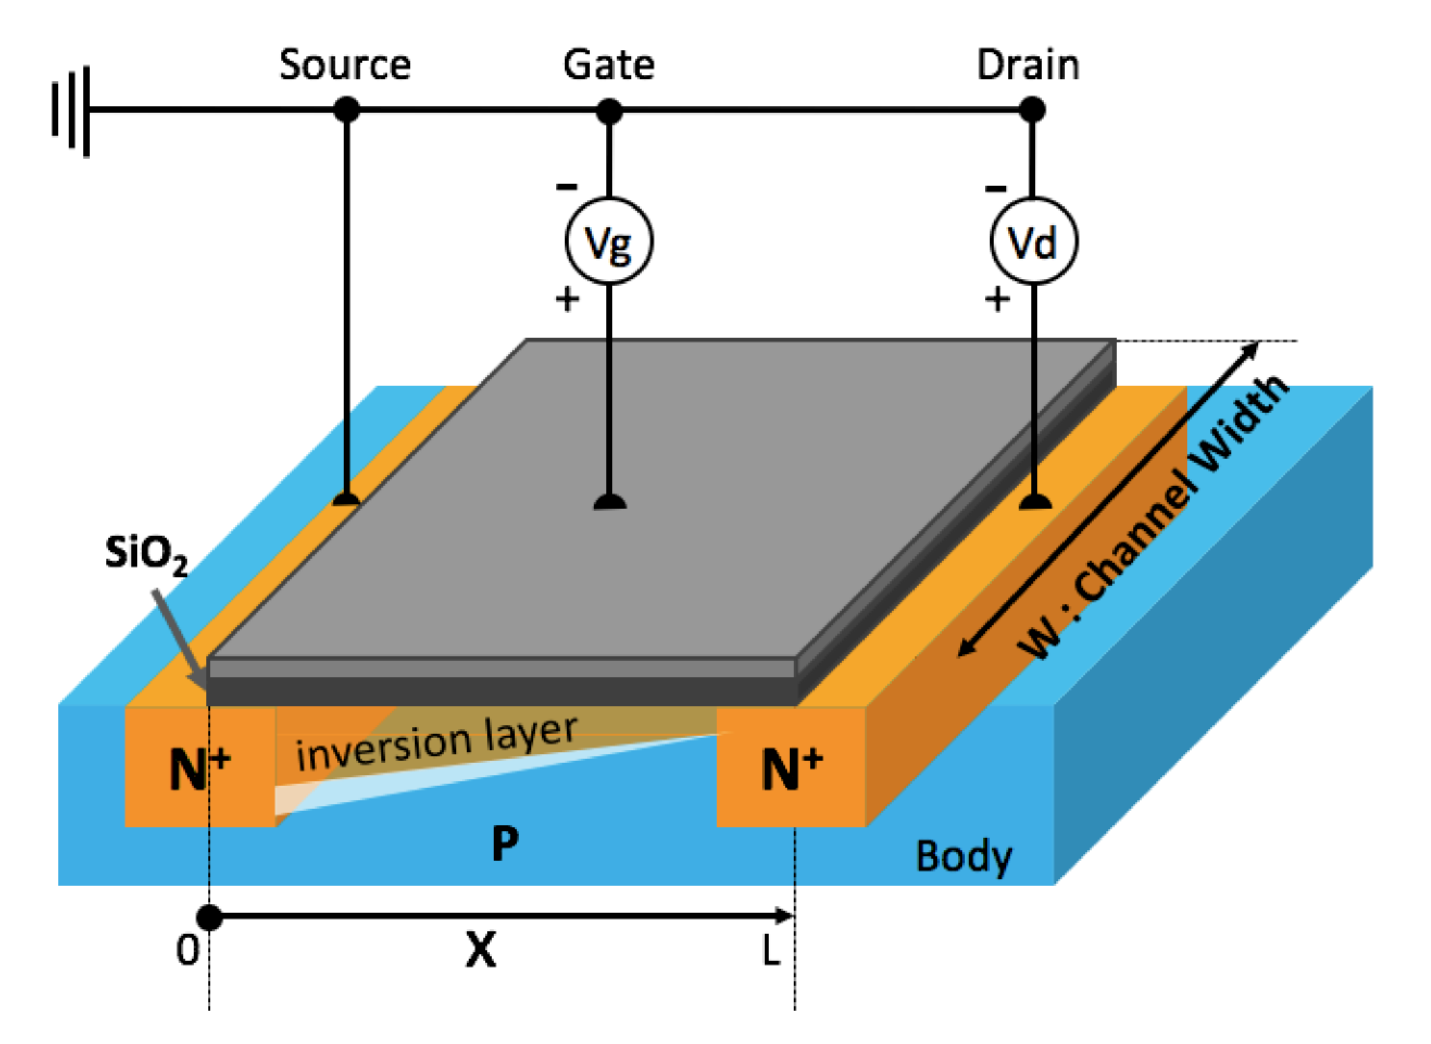
\includegraphics[clip, width=4.5cm]{./Chapter/Chapter3/Picture/MOSFET_inversion.eps}
							\hspace{1.6cm} [3]反転領域
						\end{center}
					\end{minipage}
				\end{tabular}
				\caption{NMOS動作原理概念図}
				\label{fig:MOSFET_N_WorkingPrinciple}
			\end{center}
		\end{figure}
		図\ref{fig:MOSFET_N_WorkingPrinciple}にNMOSの場合の動作原理概念図を示した。
		MOSFETの各端子に電圧を印加した際、MOSFETがどのような振る舞いを示すかを述べる。
		
		ゲート電圧が負の場合、ゲート直下には正孔が誘起される。
		このときの振る舞いは図\ref{fig:MOSFET_N_WorkingPrinciple}[1]のようになり、蓄積領域と呼ばれる。
		このときドレインとソースは強く分離され電流は流れない。
		そして、ゲート電圧が正の場合、ゲート直下には電子が誘起され、誘起された電子はP型基板中の正孔と結合して空乏層が形成される。
		このときの振る舞いは図\ref{fig:MOSFET_N_WorkingPrinciple}[2]のようになり、空乏領域と呼ばれる。
		この領域でもドレイン・ソース間に電流は流れない。
		さらに、ゲート電圧を上昇させると、ゲート直下に誘起される電子密度がP型基板の正孔密度を上回り、その結果ゲート直下の半導体の型がP型からN型へ反転した状態になる。
		この層のことを反転層と呼ぶ。
		このときの振る舞いは図\ref{fig:MOSFET_N_WorkingPrinciple}[3]のようになり、反転領域と呼ばれる。
		このときソースとドレインは反転したN型半導体で繋がれた状態になり、ドレインからソースへ電子の移動が可能になる。このときの電子(キャリア)の通り道のことをチャネルと呼ぶ。
		この結果ソースからドレインへ電流が流れるようになり、このときにMOSFETはONになる。
		そして更にゲート電圧を上昇させると、反転層が厚くなるのでより電流が流れるようになる。
		
		しかし、ゲート電圧を上げ過ぎると、ゲート酸化膜が壊れてしまう危険性がある。このゲート酸化膜は静電気でも壊れてしまう。
		したがって、電圧を印加する際や保管の際は十分注意が必要である。
		MOSFETの保管の際は静電気による絶縁破壊を防ぐために各端子をショートさせて保管する。
		そして実際にMOSFETを動作させるときは静電気バンド等を用いてしっかり静電気対策を行う必要がある。
		本節ではMOSFETのドレイン電流と各端子に印加する電圧依存性について詳しく述べる。
	\subsection{MOSFETの電流電圧特性}
		%=====IdVd plot(NMOS)を載せる=====%
		\begin{figure}[htbp]
			\begin{center}
				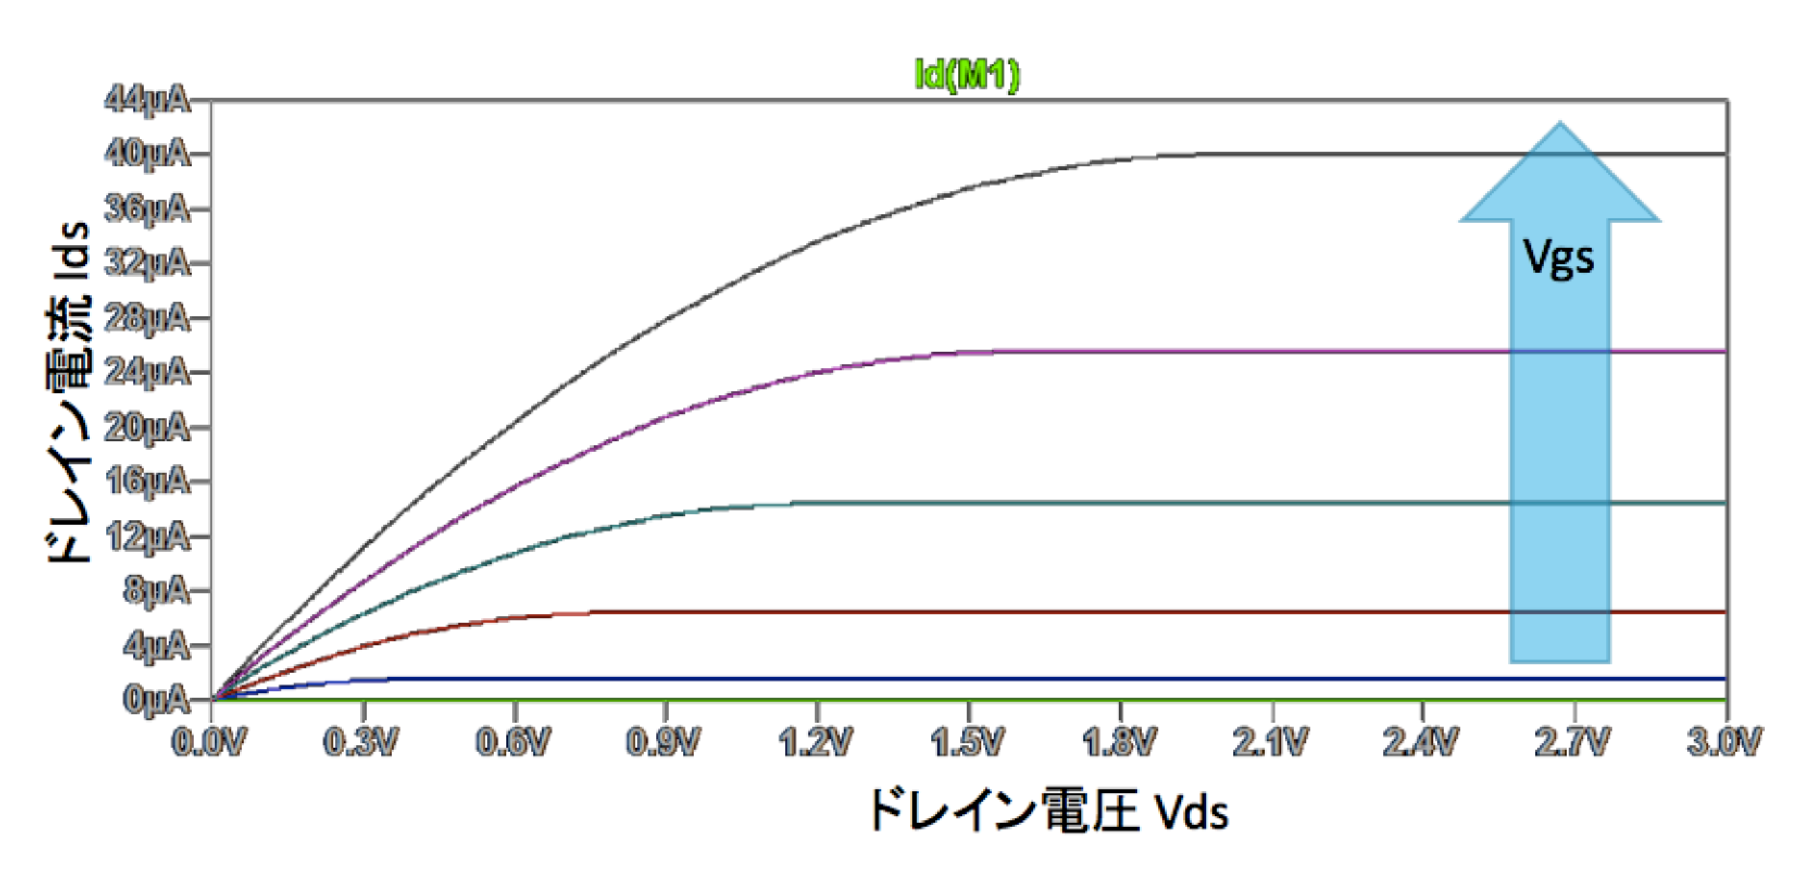
\includegraphics[width=12.0cm]{./Chapter/Chapter3/Picture/MOSFET_N_IdVd.eps}
				\caption{N型MOSFETのドレイン電流のドレイン電圧依存性}
				\label{fig:MOSFET_N_IdVd}
			\end{center}
		\end{figure}
		%=====IdVg plot(NMOS)を載せる (左 : log scale   右 : linear scale)=====%
		\begin{figure}[htbp]
			\begin{minipage}{0.5\hsize}
				\begin{center}
					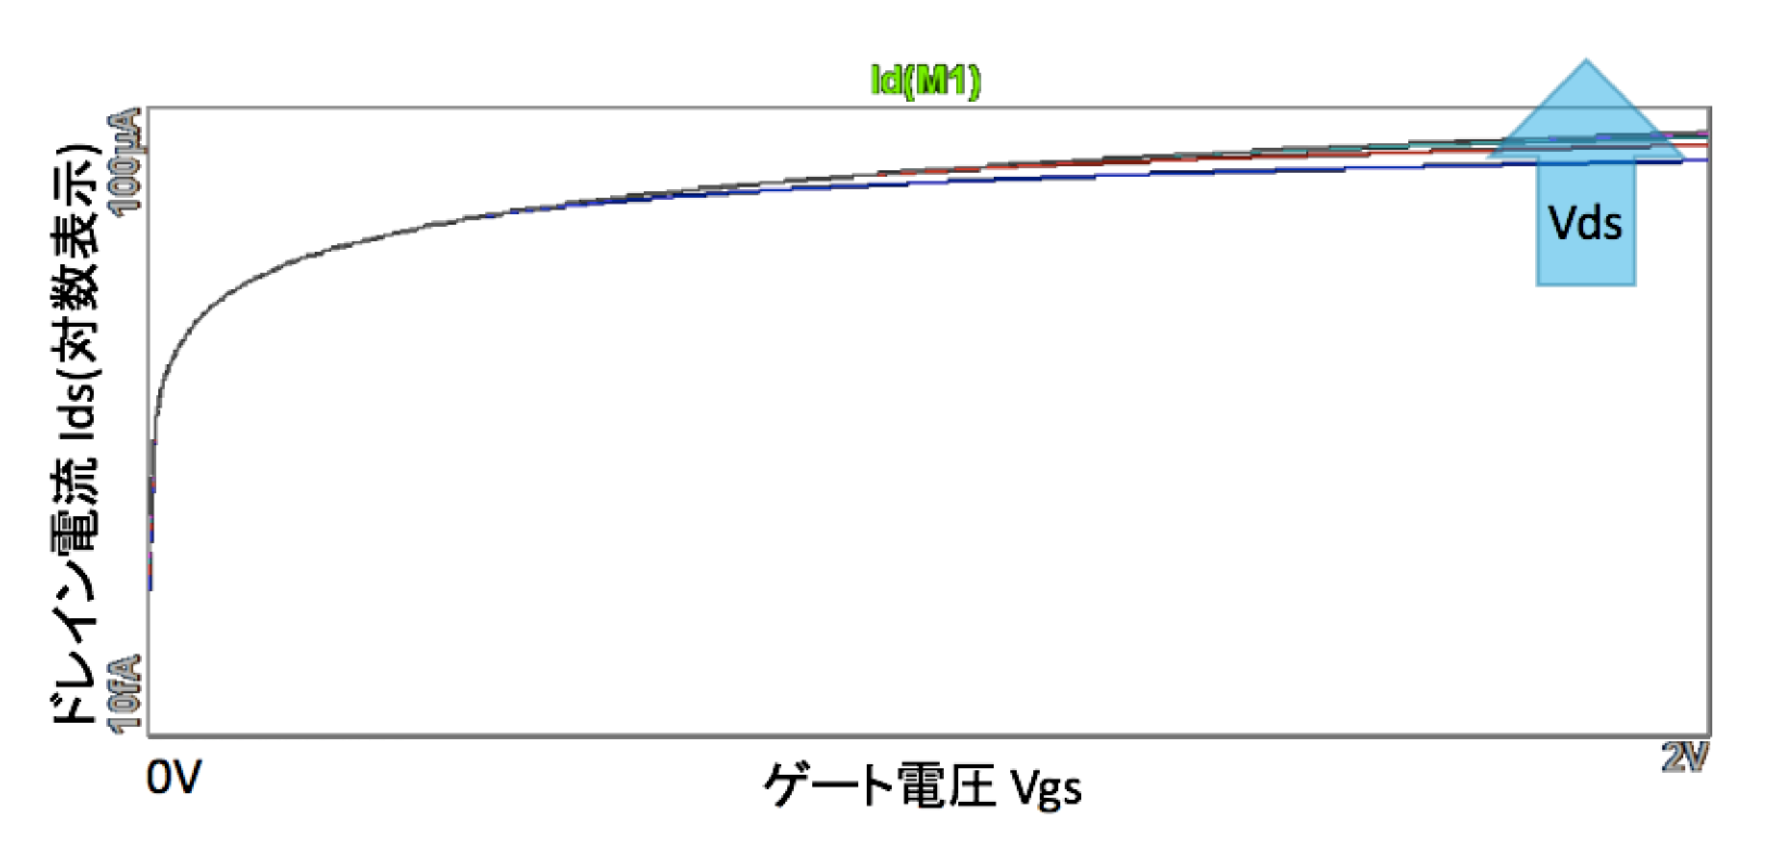
\includegraphics[width=70mm]{./Chapter/Chapter3/Picture/MOSFET_N_IdVg_log.eps}
				\end{center}
				\caption{N型MOSFETのドレイン電流のゲート電圧依存性(縦軸:対数表示)}
				\label{fig:MOSFET_N_IdVg_log}
			\end{minipage}
			\begin{minipage}{0.5\hsize}
				\begin{center}
					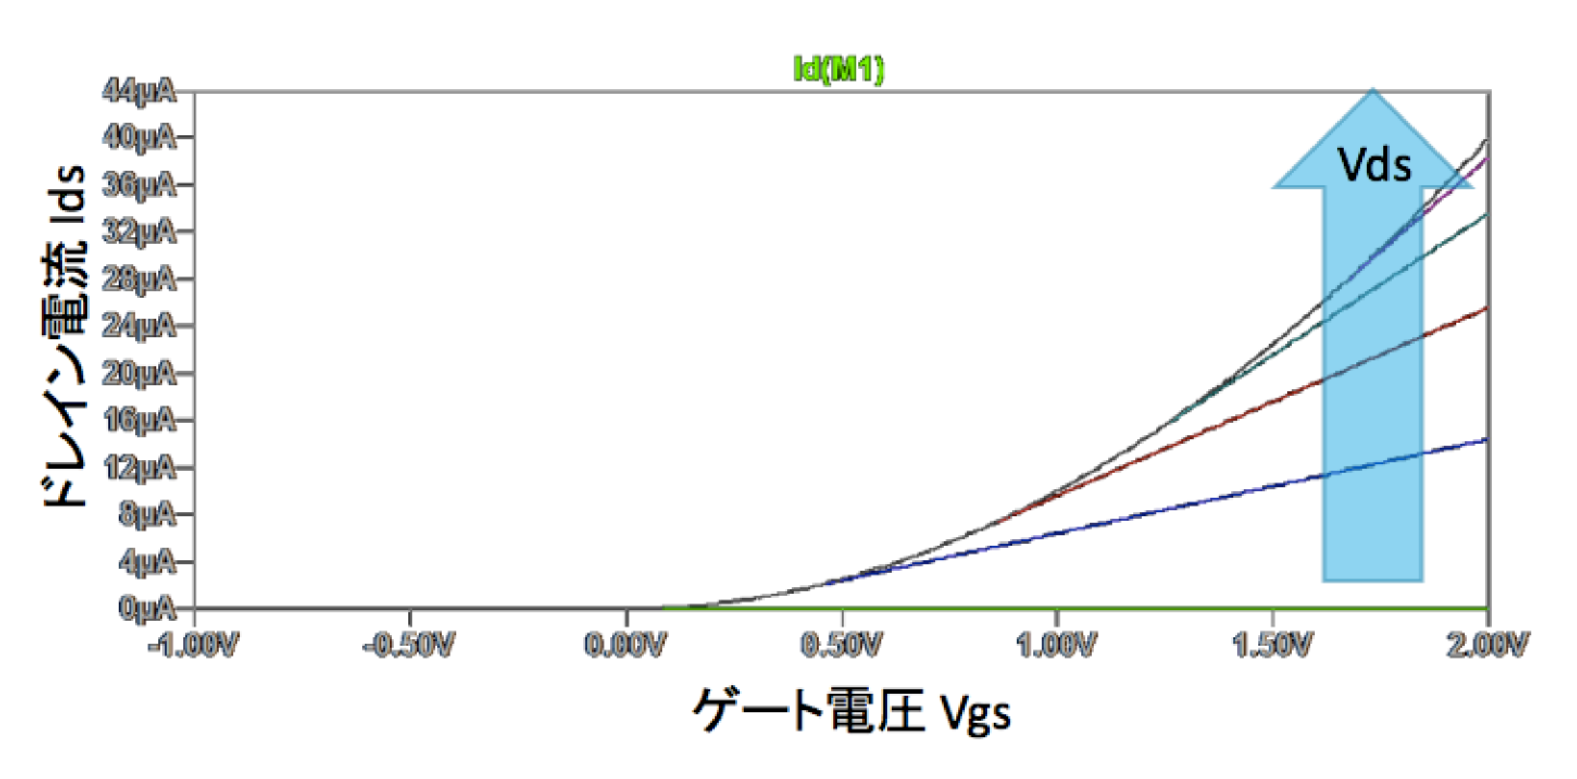
\includegraphics[width=70mm]{./Chapter/Chapter3/Picture/MOSFET_N_IdVg_linear.eps}
				\end{center}
				\caption{N型MOSFETのドレイン電流のゲート電圧依存性(縦軸:線形表示)}
				\label{fig:MOSFET_N_IdVg_linear}
			\end{minipage}
		\end{figure}
		MOSFETの電流電圧特性について、まずドレイン電流の式について述べる。ここでも前節と同様にNMOSについての場合について考える。位置$x$におけるチャネルの電子密度は閾電圧$V_{th}$以上のゲート電圧$V_{gs}$に比例しており、式(\ref{eq:MOSFET_Q})のように書ける。
		\begin{eqnarray}
			Q(x) = W C_{OX}[V_{gs} - V_{th} - V(x)]
			\label{eq:MOSFET_Q}
		\end{eqnarray}
		$W$は図\ref{fig:MOSFET_N_structure}に示したチャネル幅、$C_{OX}$は単位長さ当たりのゲート端子の電気容量、$V(x)$は位置$x$でのチャネル電位のことを指す。
		ここで電子の移動度を$\mu_{e}$とすると、ドレイン電流$I_d$は電子速度$v = \mu_{e}E$の電荷$Q(x)$の流れを表す。
		ソース・ドレイン間、つまりチャネル間の電位$E$は、
		\begin{eqnarray}
			E = \frac{dV(x)}{dx}
		\end{eqnarray}
		と表される。したがって、以上からドレイン電流$I_d$は式(\ref{eq:MOSFET_Id})のように表される。
		\begin{eqnarray}
			I_d = - \mu_e Q(x) E = - \mu_e W C_{OX}[V_{ds} - V_{th} - V(x)] \frac{dV(x)}{dx}
			\label{eq:MOSFET_Id}
		\end{eqnarray}
		以下、ゲート電圧、ドレイン電圧の関係性から2つの領域に分けて、ドレイン電流の表式について詳しく述べる。
		\subsubsection{線形領域}
			ドレイン電圧とゲート電圧の関係性が、$V_{ds} < V_{gs} - V_{th}$のときを「線形領域」と呼ぶ。
			このときチャネルはドレイン・ソース間にまたがっており、$V(L)=V_{ds}$である。
			境界条件として、$V(x=0) = 0$、$V(x=L)=V_{ds}$とする。
			式(\ref{eq:MOSFET_Id})の両辺に$dx$をかけて、積分する。
			\begin{eqnarray}
				\int_{x=0}^{x=L} I_{ds} dx = \int_{V=0}^{V=V_{ds}} W C_{OX} \mu_e [V_{ds} - V_{th} - V(x)] dV
				\label{eq:MOSFET_Id_linear1}
			\end{eqnarray}
			ドレイン電流$I_{ds}$は、位置$x=0$から$x=L$までのどの位置でも同じであることから、式(\ref{eq:MOSFET_Id_linear1})は、式(\ref{eq:MOSFET_Id_linear2})のように書くことができる。
			\begin{eqnarray}
				I_{ds} = \mu_e C_{OX} \frac{W}{L}[(V_{gs} - V_{th})V_{ds} - \frac{1}{2} {V_{ds}}^2 ]
				\label{eq:MOSFET_Id_linear2}
			\end{eqnarray}
			また、ドレイン電圧$V_{ds}$が非常に小さな領域では、ドレイン電流は以下の式(\ref{eq:MOSFET_Id_linear3})のようにドレイン電圧$V_{ds}$に対して線形近似することができる。
			\begin{eqnarray}
				I_{ds} \approx \mu_e C_{OX} \frac{W}{L} (V_{gs} - V_{th}) V_{ds}
				\label{eq:MOSFET_Id_linear3}
			\end{eqnarray}
			さらに、式(\ref{eq:MOSFET_Id_linear2})に着目すると、ドレイン電流$I_{ds}$は、$V_{ds} = V_{ds} - V_{th}$で最大値を取る。
			\begin{eqnarray}
				I_{ds} = \frac{1}{2} \mu_e C_{OX} \frac{W}{L} {(V_{gs} - V_{th})}^2
				\label{eq:MOSFET_Id_linear4}
			\end{eqnarray}
		
		\subsubsection{飽和領域}
			ドレイン電圧とゲート電圧の関係性が、$V_{ds} > V_{gs} - V_{th}$のときを「飽和領域」と呼ぶ。
			このとき、式(\ref{eq:MOSFET_Q})からわかるようにドレイン・ソース間で電荷密度がゼロになりチャネルが途切れてしまう。
			この電荷密度がゼロになってしまうことを「ピンチオフ」と呼ぶ。
			この領域でのドレイン電流$I_{ds}$の式について述べる。
			ピンチオフする位置を$x = L^{'}$とする。$V(L^{'}) = V_{gs} - V_{th}$であることに注意し、式(\ref{eq:MOSFET_Id})の両辺に$dx$をかけた式を、位置$x=0$から$x=L^{'}$まで積分する。すると式(\ref{eq:MOSFET_Id_saturate})のように書ける。
			\begin{eqnarray}
				I_{ds} = \frac{1}{2} \mu_e C_{OX} \frac{W}{L^{'}} {(V_{gs} - V_{th})}^2
				\label{eq:MOSFET_Id_saturate}
			\end{eqnarray}
			式(\ref{eq:MOSFET_Id_saturate})から、この領域においてドレイン電流$I_{ds}$はドレイン電圧$V_{ds}$に対して一定であることがわかる。
			さらに、このドレイン電流値は式(\ref{eq:MOSFET_Id_linear4})からわかるように線形領域でのドレイン電流の最大値を指す。\\
		\subsubsection{チャネル長変調効果}
			前節で、飽和領域においてドレイン電流はドレイン電圧に対して一定であると述べた。
			しかし、実際には一定ではない。\\
			ドレイン電圧$V_{ds}$が上昇すると、ドレインのN型とボディのP型によるP-N接合部分で空乏層が広がる。
			チャネルにはこの空乏層を含まないので、ドレイン側にあるピンチオフする位置がソース側にずれてしまう。
			したがって、実際にはチャネルの長さは短くなる。この効果のことを「チャネル長変調効果」という。\\
			この効果を加味したドレイン電流の式は式(\ref{eq:MOSFET_Id_channel})のようになる。
			\begin{eqnarray}
				I_{ds} \approx \frac{1}{2} \mu_e C_{OX} {(V_{gs} - V_{th})}^{2} (1 + \lambda V_{ds})
				\label{eq:MOSFET_Id_channel}
			\end{eqnarray}
			ここで、$\lambda$はチャネル長変調係数と呼ばれており、チャネル長$L$が短いほど大きくなる。
			このチャネル長変調効果は、チャネル長$L$が短いMOSFETになるほど顕著に現れる。\\
			次節では、このMOSFETを用いたアナログ回路について基礎的な部分のみ述べる。
		
\section{MOSFETを用いた回路の基礎}
	前節までは、MOSFETの各端子に印加する電圧とドレイン電流の関係性について述べた。
	本節では、このMOSFETを用いた増幅回路についての基礎について述べる。
	\subsection{トランスコンダクタンス}
		ドレイン電流はゲート・ソース間のオーバードライブ電圧$V_{\mathrm{OV}} = (V_{gs} - V_{th})$によって決まる。
		したがって、トランジスタが、入力ゲート電圧をどれだけ出力電流に変換できるかを示すことが重要である。
		ゲート電圧$V_{gs}$の変化に対するドレイン電流$I_{ds}$の変化の割合をトランスコンダクタンス($g_m$)と呼ぶ。
		式(\ref{eq:MOSFET_gm})にトランスコンダクタンス$g_m$の定義を示した。
		\begin{eqnarray}
			g_{m} & = & \left. \frac{\partial I_{ds}}{\partial V_{gs}} \right|_{V_{ds} = \mathrm{const.}}
			\label{eq:MOSFET_gm}
		\end{eqnarray}
		ここで、MOSFETの線形領域でのドレイン電流の式を示す式(\ref{eq:MOSFET_Id_linear2})に着目する。
		線形領域でのトランスコンダクタンスを計算すると以下のようになり、ゲート電圧$V_{gs}$に対して一定値を取ることがわかる。
		\begin{eqnarray}
			g_m (\mathrm{linear}) & = & \left. \frac{\partial}{\partial V_{gs}} \{ \mu_e C_{OX} \frac{W}{L} [ (V_{gs} - V_{th}) V_{ds} - \frac{1}{2} {V_{ds}}^2 ] \} \right|_{V_{ds} = \mathrm{const.}} \\
			& = & \mu_e C_{OX} \frac{W}{L} V_{ds}
		\end{eqnarray}
		
	\subsection{ドレインコンダクタンス}
		図\ref{fig:MOSFET_N_IdVd}のドレイン電流のドレイン電圧依存性に着目する。
		ドレイン電圧が低い領域では、ドレイン電流はドレイン電圧に対して一次関数的に増加し、オーバードライブ電圧$V_{OV}$以上になるとドレイン電流はほぼ一定になる。
		しかし、実際はチャネル長変調の効果により、ドレイン電流は僅かながらドレイン電圧に対して一次的に増加する。
		ドレイン電圧$V_{ds}$の変化に対するドレイン電流$I_{ds}$の変化の割合の逆数をドレインコンダクタンス$g_d$と呼ぶ。
		また、ドレインコンダクタンスの逆数のことをドレイン抵抗$r_d$と呼ぶ。
		\begin{eqnarray}
			g_d & = & \left. \frac{\partial I_{ds}}{\partial V_{ds}} \right|_{V_{gs} = \mathrm{const.}} \\
			\label{eq:MOSFET_gd_1}
			r_d & = & \frac{1}{g_d}
			\label{eq:MOSFET_gd_2}
		\end{eqnarray}
		またそれぞれのMOSFETの動作領域ごとにドレイン抵抗について述べる。
		\begin{description}
			\item[線形領域]\mbox{}\\
				線形領域でのドレイン電流の式は式(\ref{eq:MOSFET_Id_linear3})に示した。それを式(\ref{eq:MOSFET_gd_1})と式(\ref{eq:MOSFET_gd_2})に代入する。
				\begin{eqnarray}
					r_d = \frac{1}{\mu_e C_{OX} \frac{W}{L} (V_{gs} - V_{th})}
					\label{eq:MOSFET_rd_linear}
				\end{eqnarray}
				線形領域でのドレイン抵抗はオーバードライブ電圧$V_{OV}$によって制御することができる。
			\item[飽和領域]\mbox{}\\
				飽和領域でのドレイン電流(チャネル長変調効果を含む)の式は式(\ref{eq:MOSFET_Id_channel})に示した。
				前述と同様にそれを式(\ref{eq:MOSFET_gd_1})と式(\ref{eq:MOSFET_gd_2})に代入する。
				\begin{eqnarray}
					r_d = \frac{1}{\frac{1}{2} \mu_e C_{OX} \frac{W}{L} {(V_{gs} - V_{th})}^2 \lambda}
					\label{eq:MOSFET_rd_saturate}
				\end{eqnarray}
				式(\ref{eq:MOSFET_rd_saturate})より、飽和領域においてドレイン抵抗はチャネル長変調係数$\lambda$に反比例していることがわかる。
				チャネル長変調係数$\lambda$はチャネル長が長いほど小さくなるので、つまりチャネル長が長いほどドレイン抵抗は大きくなる。
		\end{description}
		次節では、これまでのMOSFETの電気的特性を踏まえ、MOSFETを用いた増幅回路について述べる。
	\subsection{MOSFETを用いた増幅回路}
		本節ではMOSFETを用いた増幅回路として、「ソース接地回路」と「ソースフォロア」の2種類の基本増幅回路について述べる。
		\subsubsection{ソース接地回路}
			\begin{figure}[htbp]
				 \begin{minipage}{0.5\hsize}
					\begin{center}
						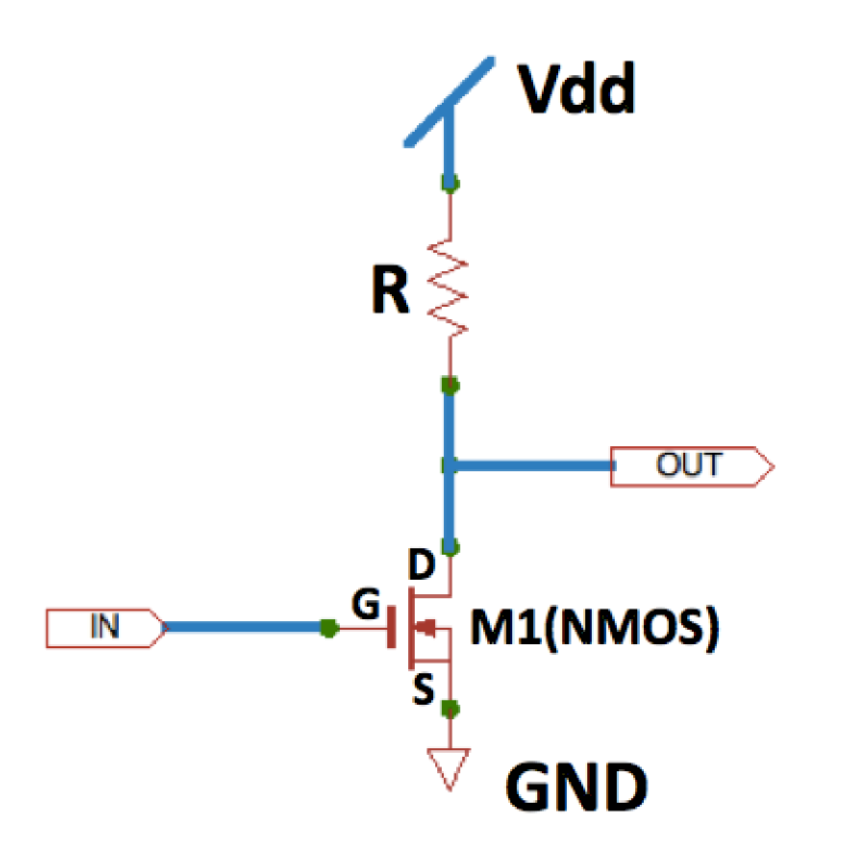
\includegraphics[width=70mm]{./Chapter/Chapter3/Picture/MOSFET_CommonSource_1.eps}
					\end{center}
					\caption{抵抗負荷を有するソース接地回路図}
					\label{fig:MOSFET_CommonSource_1}
				\end{minipage}
				\begin{minipage}{0.5\hsize}
					\begin{center}
						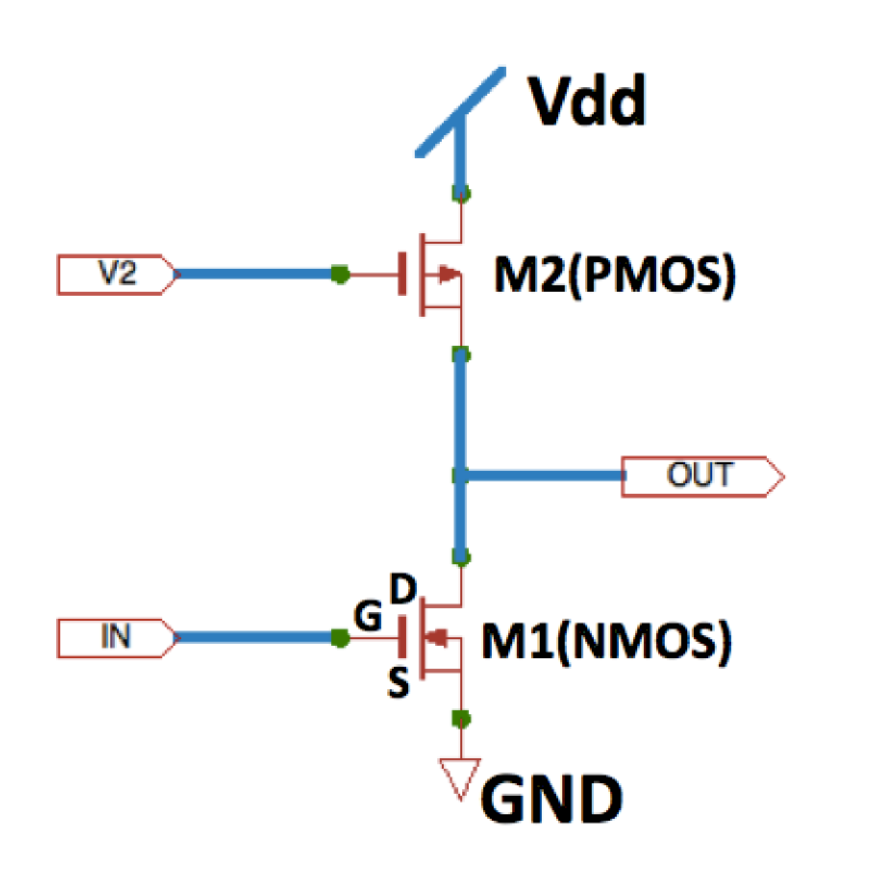
\includegraphics[width=70mm]{./Chapter/Chapter3/Picture/MOSFET_CommonSource_2.eps}
					\end{center}
					\caption{MOSFETを電流源負荷として有するソース接地回路図}
					\label{fig:MOSFET_CommonSource_2}
				\end{minipage}
			\end{figure}	
			MOSFETを用いた基本的な増幅回路として、まず「ソース接地回路」について説明する。
			図\ref{fig:MOSFET_CommonSource_1}と図\ref{fig:MOSFET_CommonSource_2}にソース接地回路図を載せる。
			まず、抵抗負荷を有する場合のソース接地回路についてに着目する。
			入力電圧($V_{IN}$)をゼロから増加させることを考える。
			はじめはM1はオフなので、M1にドレイン電流は流れない。したがって、抵抗Rでの電圧降下はないので、$V_{OUT}=V_{dd}$である。
			入力電圧$V_{IN}$が、$V_{th} + V_{OUT} > V_{IN} > V_{th}$であるとき、M1は飽和領域で動作する。
			したがって、このときの出力電圧は式{\ref{eq:MOSFET_CommonSource_1_1}}のようになる。
			ただし、ここではチャネル長変調効果を無視した。
			\begin{eqnarray}
				V_{OUT} = V_{dd} - R \frac{1}{2} \mu_e C_{OX} \frac{W}{L} {(V_{IN} - V_{th})}^2
				\label{eq:MOSFET_CommonSource_1_1}
			\end{eqnarray}
			さらに、入力電圧$V_{IN}$が、$V_{IN} > V_{OUT} + V_{th}$であるとき、M1は飽和領域を外れて線形領域で動作することになる。
			この領域において、式(\ref{eq:MOSFET_rd_linear})のようにMOSFETは抵抗のように振る舞う。
			したがって、出力電圧$V_{OUT}$は、抵抗RとMOSFETのドレイン抵抗とで抵抗分割した電圧に相当する。
			\begin{eqnarray}
				V_{OUT} = \frac{r_d (\mathrm{linear})}{rd (\mathrm{linear}) + R} V_{dd} = \frac{V_{dd}}{1 + \mu_e C_{OX} \frac{W}{L} R (V_{IN} - V_{th})}
			\end{eqnarray}
			%=====入力電圧と出力電圧の関係を示した図を載せる=====%
			\begin{figure}[htbp]
				\begin{center}
					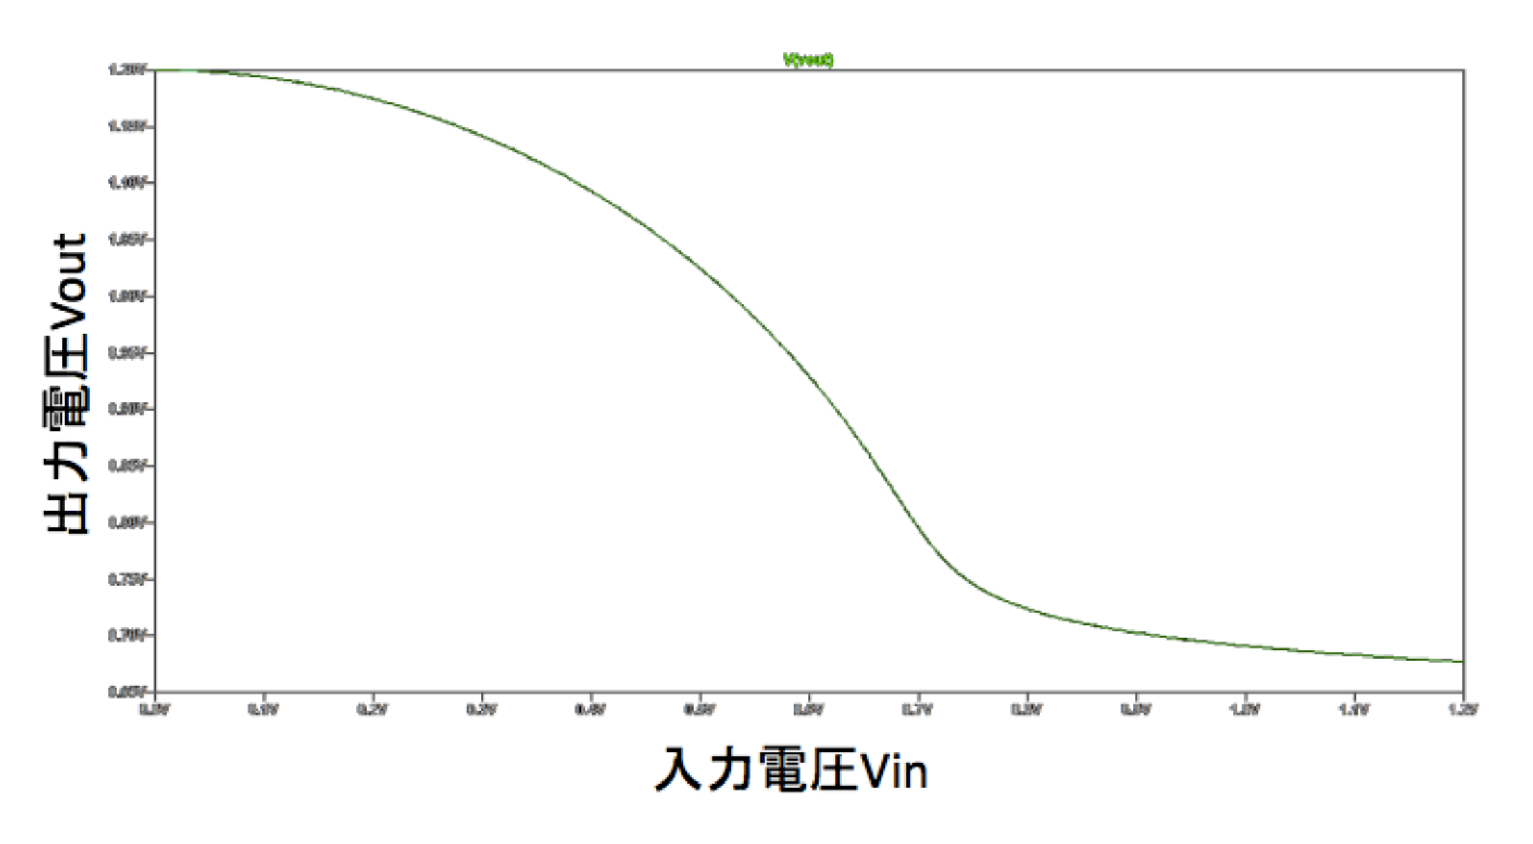
\includegraphics[width=12.0cm]{./Chapter/Chapter3/Picture/MOSFET_CommonSource_InOut.eps}
					\caption{ソース接地回路における入力電圧と出力電圧の特性}
					\label{fig:MOSFET_CommonSource_InOut}
				\end{center}
			\end{figure}
			以上より、ソース接地回路における入力電圧と出力電圧の関係性は図\ref{fig:MOSFET_CommonSource_InOut}のようになる。
			
			次に、利得について述べる。
			M1が飽和領域で動作して、かつMOSFETのチャネル長変調効果を無視しない場合、出力電圧$V_{OUT}$は式(\ref{eq:MOSFET_CommonSource_out_saturate})のように書ける。
			\begin{eqnarray}
				V_{OUT} = V_{dd} - R \frac{1}{2} \mu_e C_{OX} \frac{W}{L} {(V_{IN} - V_{th})}^2 {(1 + \lambda V_{OUT})}
				\label{eq:MOSFET_CommonSource_out_saturate}
			\end{eqnarray}
			式(\ref{eq:MOSFET_CommonSource_out_saturate})の両辺を入力電圧$V_{IN}$で微分する。
			\begin{eqnarray}
				\frac{\partial V_{OUT}}{\partial V_{IN}}
				= -R \mu_e C_{OX} \frac{W}{L} (V_{IN} - V_{th}) (1 + \lambda V_{OUT})
				- R \frac{1}{2} \mu_e C_{OX} \frac{W}{L} {(V_{IN} - V_{th})}^{2} \lambda \frac{\partial V_{OUT}}{\partial V_{IN}}
				\label{eq:MOSFET_CommonSource_out_saturate_2}
			\end{eqnarray}
			そして、$I_{ds} \approx \frac{1}{2} \mu_e C_{OX} \frac{W}{L} {(V_{IN} - V_{th})}^2$という近似を用いて、式(\ref{eq:MOSFET_CommonSource_out_saturate_2})を整理すると、電圧利得$A_{\nu}$は式(\ref{eq:MOSFET_CommonSource_out_saturate_3_1})と式(\ref{eq:MOSFET_CommonSource_out_saturate_3_2})のようになる。
			\begin{eqnarray}
				A_{\nu} & = & \frac{\partial V_{OUT}}{\partial V_{IN}} \\
				\label{eq:MOSFET_CommonSource_out_saturate_3_1}
				A_{\nu} & = & - \frac{g_m R}{1 + R \lambda I_{ds}}
				\label{eq:MOSFET_CommonSource_out_saturate_3_2}
			\end{eqnarray}
			そして、$\lambda I_{ds} = \frac{1}{r_{d} (\mathrm{saturate})}$なので、
			\begin{eqnarray}
				A_{\nu} = - g_{m} \frac{r_{d}(\mathrm{saturate}) R}{r_{d}(\mathrm{saturate}) + R}
				\label{eq:MOSFET_CommonSource_out_saturate_4}
			\end{eqnarray}
			式(\ref{eq:MOSFET_CommonSource_out_saturate_4})から、負荷抵抗Rが大きければ大きいほど電圧利得$A_{\nu}$は大きくなることがわかる。\\
			図\ref{fig:MOSFET_CommmonSource_2}にMOSFETを電流源負荷として用いたソース接地回路図を示した。
			抵抗素子の代わりにMOSFETを電流源として用いることによって、
			\begin{itemize}
				\item 一般的なCMOS技術では高精度・高抵抗な抵抗素子を形成するのは困難だが、MOSFETを用いることで高抵抗負荷を実現できる。
				\item 供給電圧を大きく消費せずに高抵抗を実現できるので、消費電力低減が期待できる。
			\end{itemize}
		\subsubsection{ソースフォロア回路}
			\begin{figure}[htbp]
				 \begin{minipage}{0.5\hsize}
					\begin{center}
						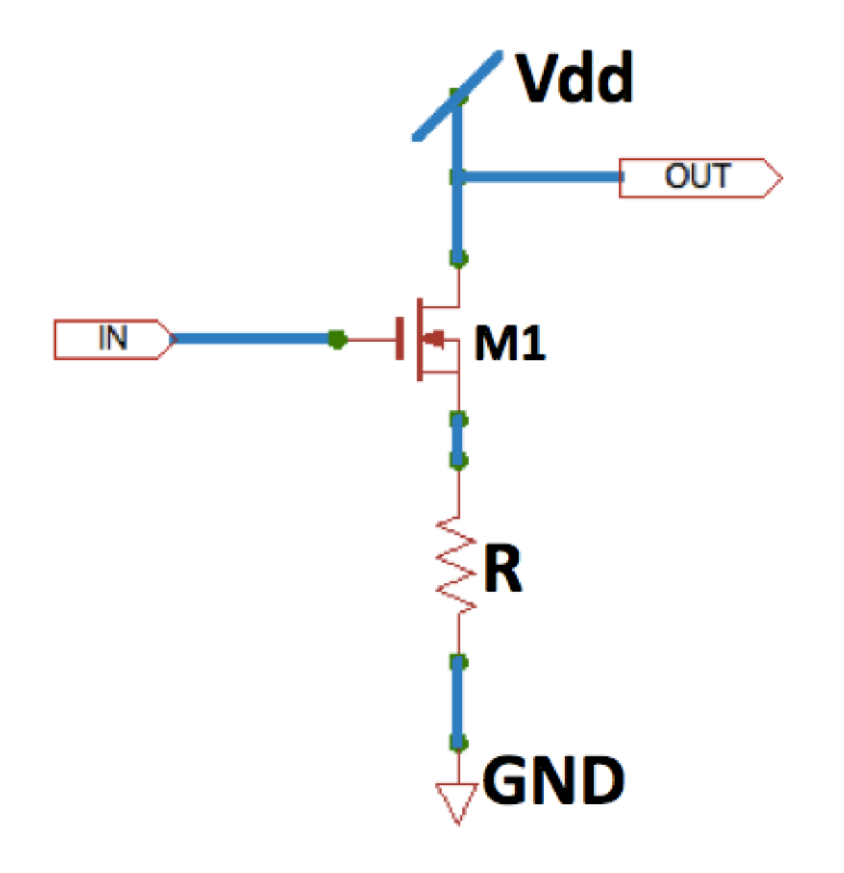
\includegraphics[width=70mm]{./Chapter/Chapter3/Picture/MOSFET_SourceFollower_1.eps}
					\end{center}
					\caption{抵抗負荷を有するソースフォロア(ドレイン接地)回路図}
					\label{fig:MOSFET_SourceFollower_1}
				\end{minipage}
				\begin{minipage}{0.5\hsize}
					\begin{center}
						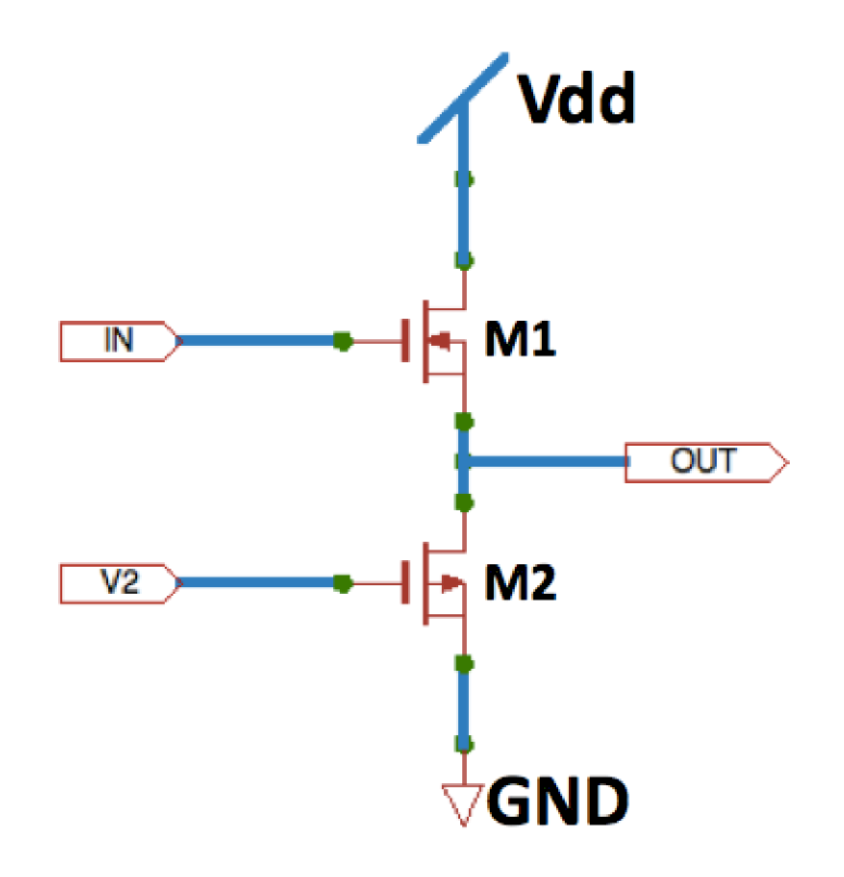
\includegraphics[width=70mm]{./Chapter/Chapter3/Picture/MOSFET_SourceFollower_2.eps}
					\end{center}
					\caption{MOSFETを電流源負荷として有するソースフォロア(ドレイン接地)回路図}
					\label{fig:MOSFET_SourceFollower_2}
				\end{minipage}
			\end{figure}	
			図\ref{fig:MOSFET_SourceFollower_1}と図\ref{fig:MOSFET_SourceFollower_2}のような回路のことをソースフォロア(ドレイン接地)回路と呼ばれる。
			前節で述べたソース接地回路において、高い電圧利得を得るためには負荷インピーダンスを大きくする必要がある。
			このような増幅段が低インピーダンスの負荷を駆動する場合は、信号電圧の損失が無視できるようにバッファを入れる必要がある。
			ソースフォロア回路は、このバッファとしての役割を果たす。\\
			%=====入力電圧と出力電圧の関係を示した図を載せる=====%
			\begin{figure}[htbp]
				\begin{center}
					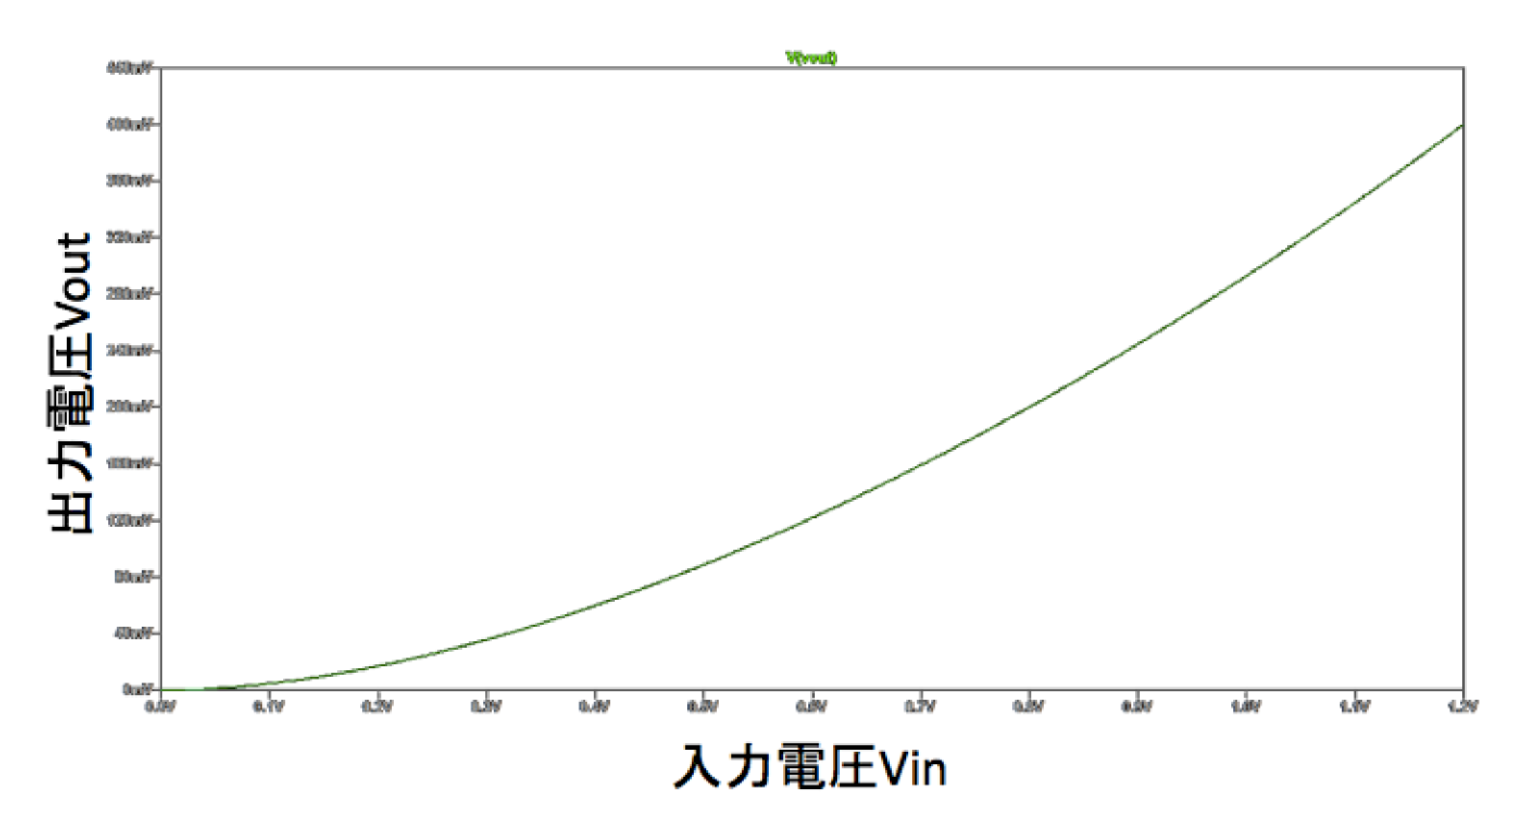
\includegraphics[width=12.0cm]{./Chapter/Chapter3/Picture/MOSFET_SourceFollower_InOut.eps}
					\caption{ソースフォロア回路における入力電圧と出力電圧の特性}
					\label{fig:MOSFET_SourceFollower_InOut}
				\end{center}
			\end{figure}
			次に前節の時と同様に、入力電圧$V_{IN}$をゼロから増加させることを考える。\\
			入力電圧$V_{IN}$が、$V_{IN} < V_{th}$ではM1はオフなので出力電圧$V_{OUT}=0$である。\\
			そして、入力電圧$V_{IN}$が、$V_{IN} > V_{OUT}$になると、M1は飽和領域で動作する
			\footnote{$V_{dd}$の値によってはM1は線形領域で動作することにもなるが、基本的にはM1は飽和領域で動作するよう$V_{dd}$を印加する。}。
			M1が飽和領域で動作していることから、ソースフォロア回路における入出力電圧の特性は式(\ref{eq:MOSFET_SourceFollower_InOut})のように書くことができる。
			\begin{eqnarray}
				V_{OUT} = \frac{1}{2} \mu_e C_{OX} \frac{W}{L} {(V_{IN} - V_{th} - V_{OUT})}^2 R
				\label{eq:MOSFET_SourceFollower_InOut}
			\end{eqnarray}
			これをグラフにすると図\ref{fig:MOSFET_SourceFollower_InOut}のようになる。\\
			次にソースフォロアの電圧利得について考える。
			式(\ref{eq:MOSFET_SourceFollower_InOut})の両辺を出力電圧$V_{IN}$で微分する。
			\begin{eqnarray}
				\frac{\partial V_{OUT}}{\partial V_{IN}} = \frac{1}{2} \mu_e C_{OX} \frac{W}{L} 2 (V_{IN} - V_{th} - V_{OUT}) \left( 1 - \frac{\partial V_{th}}{\partial V_{IN}} \right) R
				\label{eq:MOSFET_SourceFollower_1}
			\end{eqnarray}
			そして、
			\begin{eqnarray}
				\frac{\partial V_{th}}{\partial V_{IN}} = \eta \frac{\partial V_{OUT}}{\partial V_{IN}}
			\end{eqnarray}
			であることから、電圧利得$A_{\nu}$は式(\ref{eq:MOSFET_SourceFollower_2_1})と式(\ref{eq:MOSFET_SourceFollower_2_2})のようになる。
			\begin{eqnarray}
				A_{\nu} & = & \frac{\partial V_{OUT}}{\partial V_{IN}} \\
				\label{eq:MOSFET_SourceFollower_2_1}
				A_{\nu} & = & \frac{\mu_e C_{OX} \frac{W}{L} (V_{IN} - V_{th} - V_{OUT}) R}{1 + \mu_e C_{OX} \frac{W}{L} (V_{IN} - V_{th} - V_{OUT}) R (1 + \eta)}
				\label{eq:MOSFET_SourceFollower_2_2}
			\end{eqnarray}
			トランスコンダクタンス$g_m$は、
			\begin{eqnarray}
				g_m = \mu_e C_{OX} \frac{W}{L} (V_{IN} - V_{th} - V_{OUT})
			\end{eqnarray}
			であることから、トランスコンダクタンスが大きいほど増幅率は1に近づく。
			そしてソースフォロア回路はソース接地回路と同様に負荷抵抗の代わりにMOSFETを電流源として用いる。
			\clearpage
\section{SOI-MOSFET}
	前節まではMOSFETの電気的特性やMOSFETを用いた基本的な増幅回路について述べた。
	本節ではMOSFETの構造について、まず一般的なBulk-CMOSの構造について述べる。
	Bulk-CMOSとはシリコンSiバルク上にMOSFETが形成された構造を呼ぶ。
	
	対して、SOI(Silicon On Insulator)-MOSFETと呼ばれるMOSFETがある。これは$\mathrm{SiO_2}$酸化膜上に形成されたMOSFETである。\\
	このSOI-MOSFETの中でもチャネル層が非常に薄く形成されたFD(Fully Depleted)-SOI-MOSFETは4Kで動作したことが確認されている。\\
	本節ではこのSOI-MOSFETの極低温特性についても詳しく述べる。
	\subsection{CMOS}
		\begin{figure}[htbp]
			\begin{center}
				\includegraphics[width=12.0cm]{./Chapter/Chapter3/Picture/CMOS_structure.eps}
				\caption{Bulk-CMOSの構造}
				\label{fig:CMOS_structure}
			\end{center}
		\end{figure}
		1つの基板上に複数のMOSFETを集積して組み合わせた構造のことをCMOS(Complementary MOS)と呼ばれる。
		通常のBulk CMOSは基板とデバイス同士がPN接合の逆バイアス電圧によって分離される。
		Bulk-CMOSの構造は図\ref{fig:CMOS_structure}に示した。
		
		しかしこれでは素子同士の分離は完全ではない。
		SOIプロセスで形成されたMOSFETでは、より素子同士の分離が完全になる。
		
	\subsection{PD-SOI-FETとFD-SOI-FET}
		\begin{figure}[htbp]
			\begin{center}
				\includegraphics[width=12.0cm]{./Chapter/Chapter3/Picture/SOIFET_structure.eps}
				\caption{SOI-CMOSの構造(左 : FD-SOI-MOSFET    右 : PD-SOI-MOSFET)}
				\label{fig:SOIFET_structure}
			\end{center}
		\end{figure}
		SOIプロセスによって形成されたMOSFETは素子同士を絶縁膜である$\mathrm{SiO_2}$で完全に電気的に分離する。
		
		我々のCOBAND実験において、Bulk-CMOSよりもSOI-CMOSの方が優れている点として以下の3点が挙げられる。
		\begin{description}
			\item[集積化に非常に優れている]\mbox{}\\
				絶縁膜により素子を完全に電気的に分離しているので、素子間のクロストークが非常に小さいので集積化に優れている。
			\item[低消費電力化が可能]\mbox{}\\
				Bulk-CMOSの場合、基板と各端子間との寄生容量が生じてしまう。
				対してSOI-CMOSの場合はそれに起因する寄生容量を抑えることができる。
			\item[回路の高速化が可能]\mbox{}\\
				前述と同様、寄生容量を抑えられるので、低消費電力化と同時に高速化も期待される。
		\end{description}
		そしてSOI-MOSFETは、ゲート直下のチャネル層の厚みにより、
		\begin{description}
		\item[部分空乏型SOI(PD-SOI : Partially Depleted SOI)]\mbox{}\\
			SOI層の厚みはおよそ100nm〜200nm程度。\\
			チャネル層が厚いのでゲート電圧を印加してもゲート直下のみが部分的に空乏化され、電気的に中性な領域(Body)が現れる。
		\item[完全空乏型SOI(FD-SOI : Fully Depleted SOI)]\mbox{}\\
			SOI層の厚みは50nm以下でPD-SOIプロセスで形成されてMOSFETよりも非常に薄い。\\
			チャネル層が薄いのでゲート直下のシリコン層は完全に空乏化する。
		\end{description}
		に大別される。
		
		特にFD-SOIプロセスで形成されたMOSFETは浮遊帯効果を抑制でき、我々が極低温環境下で動作させるのに最大のメリットが発揮される。
		
		浮遊帯効果とはMOSFETが動作している際、そのキャリアの衝突イオン化により生成された正孔がBody部分に蓄積し、結果Body電位が変化するのでMOSFETが誤作動を起こしてしまう効果のことである。
		低温環境下においてキャリア移動度が上昇するので、この衝突イオン化が起こりやすくなる。
		したがって、極低温環境下でMOSFETを用いることを考える場合は浮遊帯効果を抑制できるようなMOSFETを用いる必要がある。
		この浮遊体効果はBulk-CMOSプロセスで形成されたMOSFETはもちろん、PD-SOIプロセスで形成されたMOSFETも浮遊帯効果により低温環境下では動作しない。
		
		しかし、FD-SOI-MOSFETはbody部分が完全に空乏化されるので浮遊帯効果は起こらない。実際、JAXAはFD-SOI-MOSFETが4Kで動作したことを確認した\cite{6}。
	\subsection{極低温特性}
		\begin{figure}[htbp]
			\begin{minipage}{0.5\hsize}
				\begin{center}
					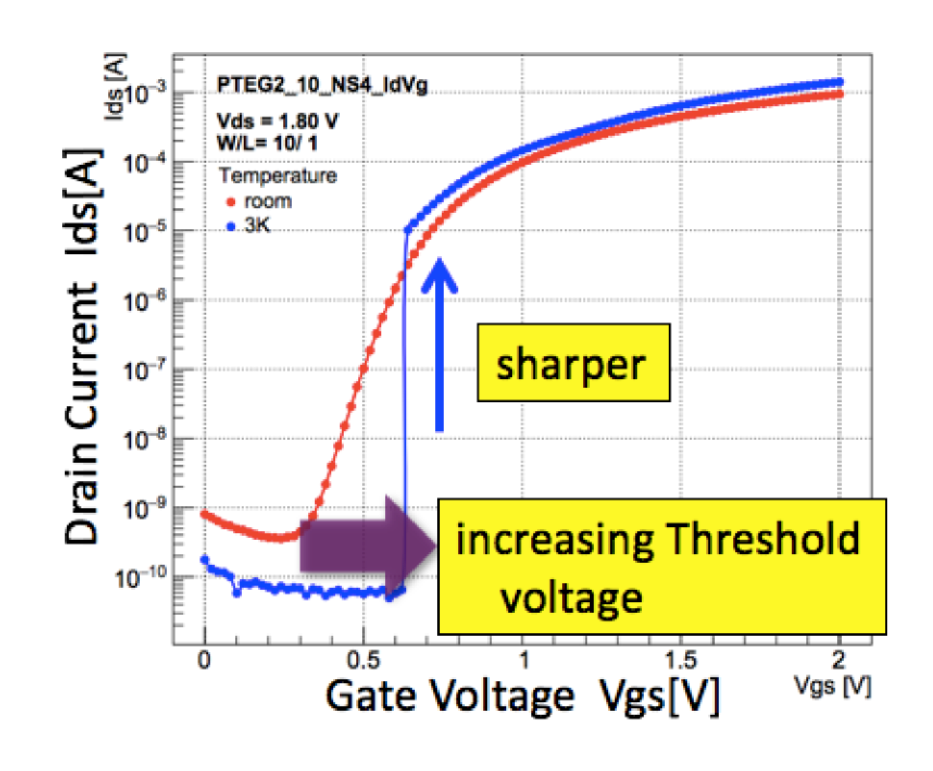
\includegraphics[width=60mm]{./Chapter/Chapter3/Picture/MOSFET_IdVg_temp.eps}
				\end{center}
				\caption{FD-SOI-MOSFETのドレイン電流の温度依存性($I_{ds} - V_{gs}$特性)}
				\label{fig:MOSFET_IdVg_temp}
			\end{minipage}
			\begin{minipage}{0.5\hsize}
				\begin{center}
					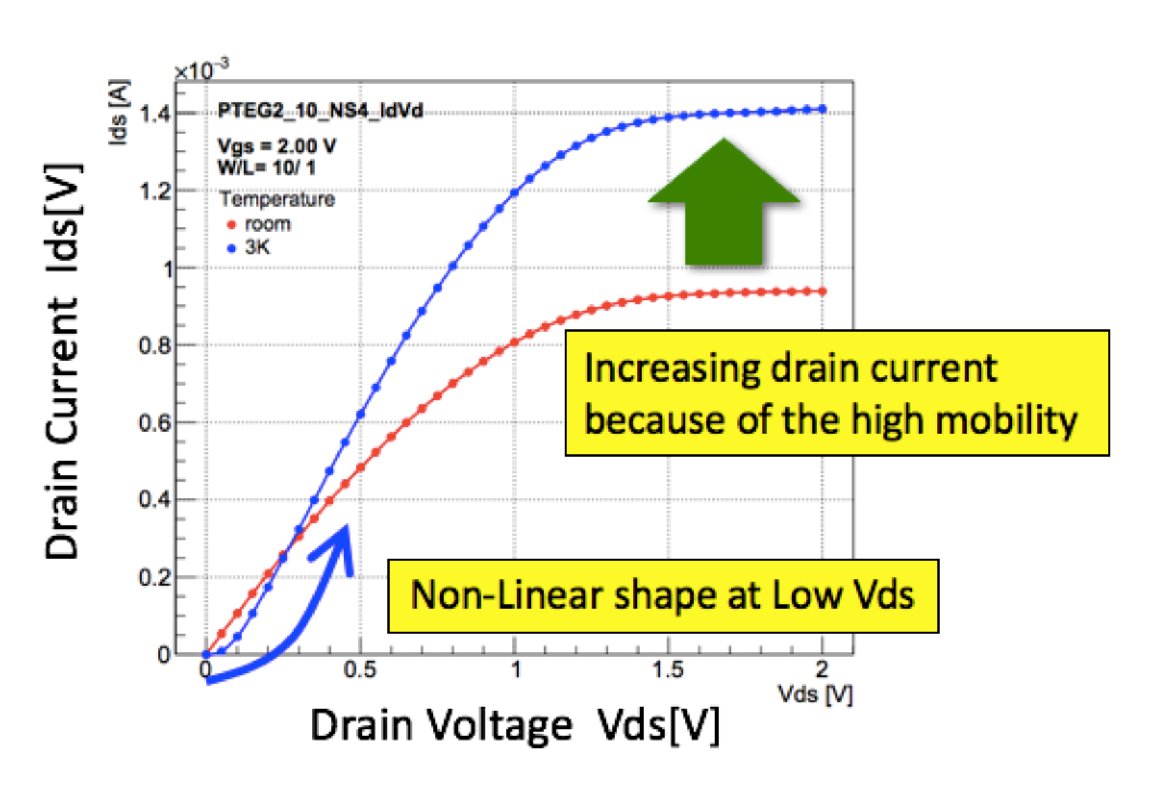
\includegraphics[width=80mm]{./Chapter/Chapter3/Picture/MOSFET_IdVd_temp.eps}
				\end{center}
				\caption{FD-SOI-MOSFETのドレイン電流の温度依存性($I_{ds} - V_{ds}$特性)}
				\label{fig:MOSFET_IdVd_temp}
			\end{minipage}
		\end{figure}
		FD-SOI-MOSFETのドレイン電流の温度依存性について、図\ref{fig:MOSFET_IdVg_temp}と図\ref{fig:MOSFET_IdVd_temp}に示した。
		室温時(赤点)のMOSFETの電流電圧特性と3K時(青点)のMOSFETの電流電圧特性を比較すると、極低温環境下では、
		\begin{itemize}
			\item 閾電圧の上昇
			\item サブスレッショルド領域で立ち上がりがより鋭くなる
			\item キャリア移動度上昇による飽和電流値の上昇
		\end{itemize}
		が見られる。ただし、3K環境下と300mK環境下ではFD-SOI-MOSFETの電流電圧特性の基本動作に変化はない。
		さらに、極低温環境下におけるドレイン電流のドレイン電圧特性($I_{ds}-V_{ds}$特性)に着目すると、以下のような異常特性が確認されている。
		\begin{itemize}
			\item $V_{ds}$が高い領域でドレイン電流の急激な上昇(Kink効果)
			\item $V_{ds}$が低い領域でのドレイン抵抗の異常な上昇
		\end{itemize}
		上記1つ目の異常特性によって、Kink効果が現れない電圧に調整することで異常特性を回避することができる。
		上記2つ目の異常特性に関してはLDD不純物濃度を濃くすることによって改善できることを確認しており、これは次章で詳しく報告する。
		
		以上のように、極低温環境下におけるFD-SOI-MOSFETの電流電圧特性は常温環境下から大きく変化するので、これらの特性変動を踏まえた上で極低温環境用の増幅器開発をする必要がある。
		\clearpage
		
\section{極低温増幅器への要求}
	我々はFD-SOI-MOSFETを用いた極低温環境用前置増幅器でNb/Al-STJ検出器信号の増幅を行う。その前置増幅器には以下の要求が課される。
	\begin{description}
		\item[Nb/Al-STJ検出器信号のような高速な信号でも増幅可能であること]\mbox{}\\
			STJ検出器の信号幅は数$\mathrm{\mu s}$から数百$\mathrm{\mu s}$程度である。
			したがって数十kHzから数MHz帯域の信号に対しても十分増幅できる回路である必要がある。
		\item[冷凍機配線容量を駆動可能]\mbox{}\\
			冷凍機配線は常温環境下からサンプルが設置された極低温環境下へ熱アンカーを取るため非常に長い。
			したがって、冷凍機の配線容量は数百pF程度で非常に大きいことが確認されている。
		\item[極低温環境下でも増幅器として動作可能であること]\mbox{}\\
			現在我々が性能評価を行っているCRAVITY製Nb/Al-STJ検出器のリーク電流は約400mK程度で下げ止まる。
			STJ検出器直近で動作させる場合は400mK以下でも動作可能な増幅器である必要がある。
		\item[400チャンネルに対して消費電力が$0.25\mathrm{W}$以下であること]\mbox{}\\
			次章で述べるが、我々が用いる冷凍機の冷却能力は350mKで100$\mathrm{\mu W}$程度である。
			もし増幅器をSTJ検出器直近で動作させる場合は、増幅器の消費電力は100$\mu W$以下である必要がある。
			しかし、現在極低温環境用前置増幅器の設計において、350mKでの消費電力の要求は非常に厳しいのが現状である。
			もし増幅器をより冷却能力が高い3K環境に設置する場合、400チャンネルに対する消費電力への要求は0.25$\mathrm{W}$に軽減される。
	\end{description}
	以上の要求を満たすように我々はFD-SOI-MOSFETを用いた極低温環境用増幅器(以下、SOI増幅器と呼ぶ)の研究開発を行ってきた。
	次節から、極低温環境用前置増幅器の研究開発の現状について順を追って述べる。
	\clearpage
\section{極低温環境用SOI前置増幅器の研究開発の現状}
	現時点では、極低温環境用SOI-MOSFETのSPICE回路シミュレーターは完成していないので、前置増幅器の設計は常温環境下でのSOI-MOSFETのパラメータで行い、極低温環境下で動作させる時に各MOSFETの極低温特性を考慮し電圧設定を決定した。
	\subsection{SOI前置増幅器一体型STJ検出器}
		\begin{figure}[htbp]
			\begin{center}
				\includegraphics[width=12.0cm]{./Chapter/Chapter3/Picture/SOISTJ_structure.eps}
				\caption{SOI前置増幅器一体型STJ検出器(SOI-STJ)の構造概念図}
				\label{fig:SOISTJ_structure}
			\end{center}
		\end{figure}
		前章で、STJ検出器が動作する極低温環境下においても動作可能な前置増幅器を冷凍機内に設置し、STJ検出器信号が冷凍機の長い配線を経て読み出す際に生じる雑音に埋もれる前に増幅させるようと考えていることを述べた。
		出来るだけSOI増幅器をSTJ検出器に近づければ、冷凍機配線に起因する測定系雑音の影響を回避して増幅することができる。
		究極的にはSOI増幅器回路基板上にSTJ検出器を直接形成した増幅器と検出器が一体型の光検出器にすることで、冷凍機配線を介さずに増幅することが出来るので、SN比がよくなることが期待される。\\
		図\ref{fig:SOISTJ_structure}にSOI前置増幅器とSTJ検出器が一体型となった光検出器(SOI-STJ)の構造概念図を示す。SOI回路基板上に直接STJ検出器を形成している。
		回路との電気的接触はタングステンのビアを介して行われており、また回路基板の表面はCMP研磨によって平坦化を行う。\\
		SOI回路基板は株式会社ラピスセミコンダクタに制作を依頼している。
	\subsection{1号機(SOI-STJ1)}
		\begin{figure}[htbp]
			\begin{center}
				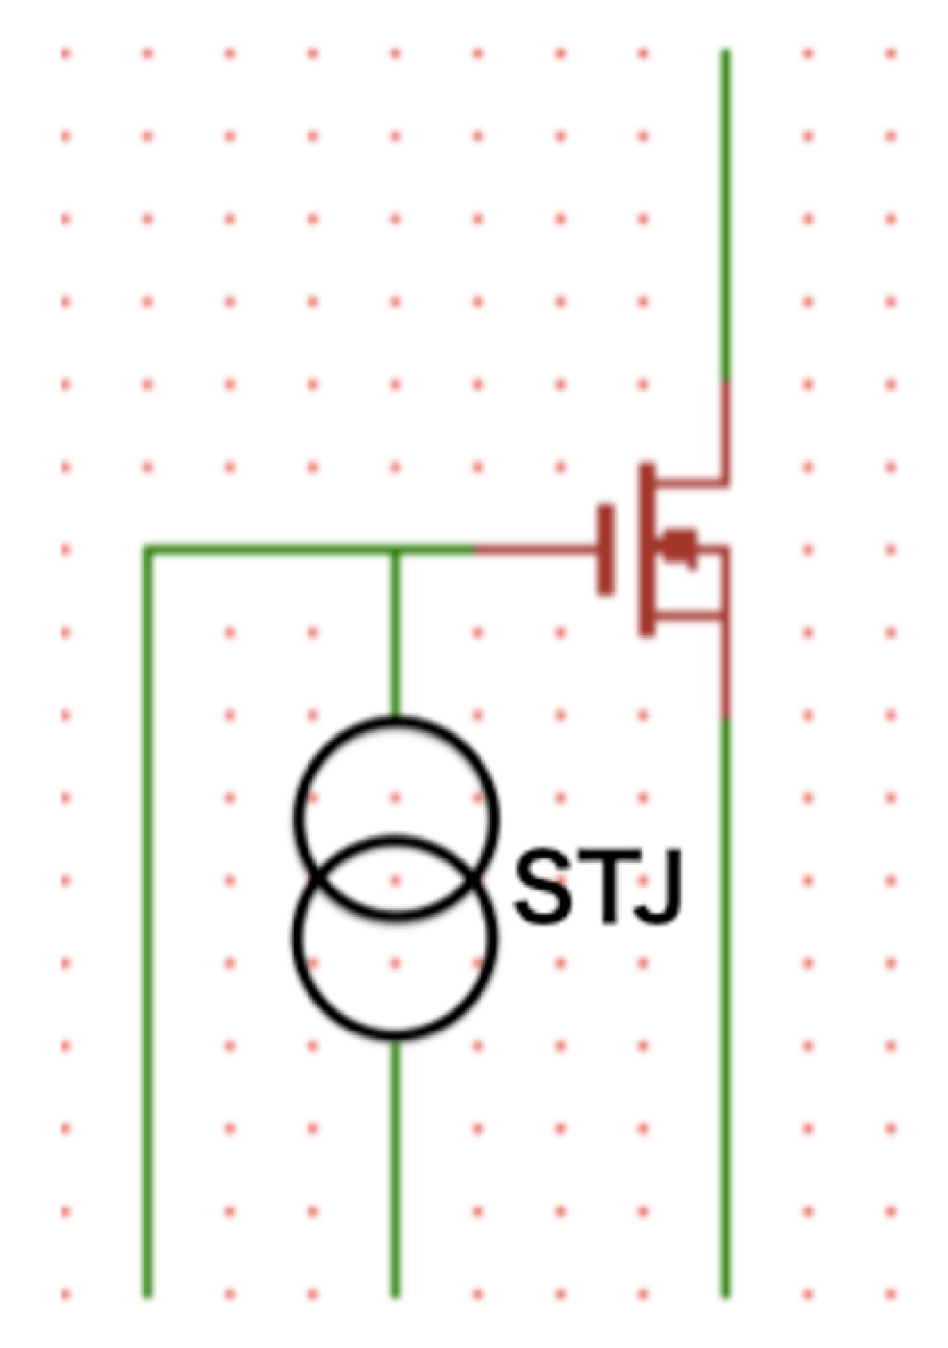
\includegraphics[width=6.0cm]{./Chapter/Chapter3/Picture/SOISTJ1_circuit.eps}
				\caption{極低温環境用SOI前置増幅器1号機(SOI-STJ1)}
				\label{fig:SOISTJ1_circuit}
			\end{center}
		\end{figure}
		試作段階として2013年度にSOI増幅器1号機(以下、SOI-STJ1)が制作された。SOI-STJ1の回路図を図\ref{fig:SOISTJ1_circuit}に示す。
		またSOI-STJ1ではFETの型に応じて2パターンの回路を用意している。それぞれの詳細については表\ref{tab:SOISTJ1_detail}に示す。
		\begin{table}[htb]
			\begin{center}
				\begin{tabular}{| l || c | c | c | c |} \hline
					\  & FET Type & Channel Width & Channel Length & Gate Cap. \\ \hline \hline
					Pattern1 & Nch & $10\mathrm{\mu m} \times 100$ & $1 \mathrm{\mu m}$ & $8 \mathrm{pF}$ \\ \hline
					Pattern2 & Pch & $10\mathrm{\mu m} \times 100$ & $1 \mathrm{\mu m}$ & $8 \mathrm{pF}$ \\ \hline
				\end{tabular}
				\caption{SOI-STJ1の各パターンごとのFETの詳細}
				\label{tab:SOISTJ1_detail}
			\end{center}
		\end{table}
		SOI回路基板上にNb/Al-STJ検出器を形成したSOI-STJ1の性能評価実験によって以下の結果が得られた。
		\begin{enumerate}
			\item SOI回路基板にNb/Al-STJ検出器を形成しても、Nb/Al-STJは損傷はなく正常に動作した。
			\item SOI-MOSFETがNb/Al-STJの動作温度(1K以下)でも正常に動作した。
		\end{enumerate}
	\subsection{2号機(SOI-STJ2)}
		\begin{figure}[htbp]
			\begin{center}
				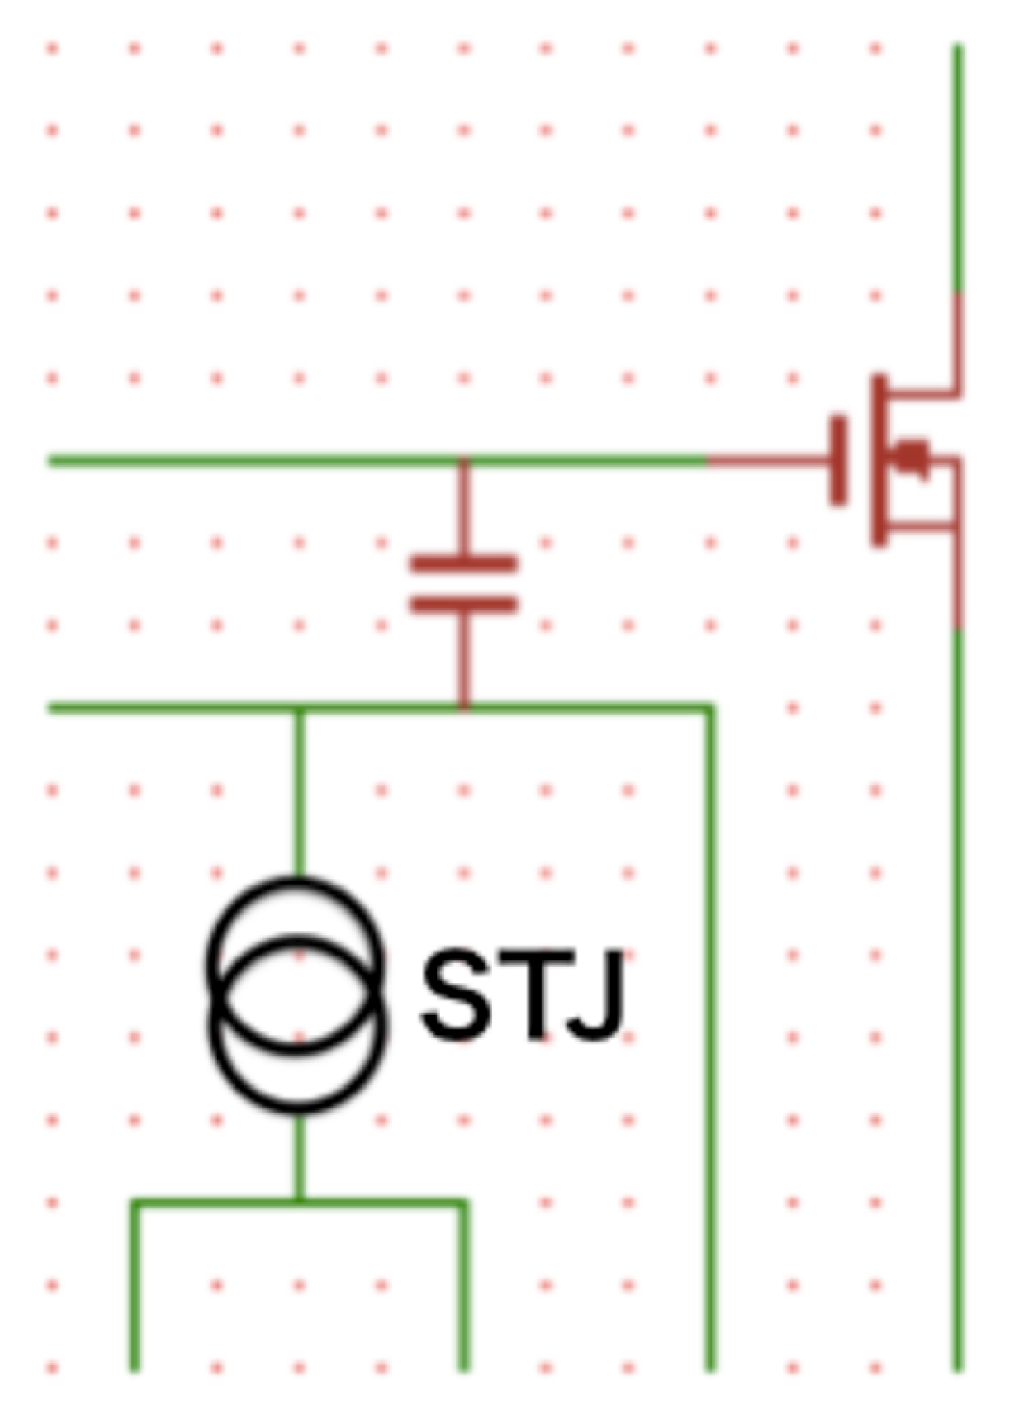
\includegraphics[width=6.0cm]{./Chapter/Chapter3/Picture/SOISTJ2_circuit.eps}
				\caption{極低温環境用SOI前置増幅器2号機(SOI-STJ2)}
				\label{fig:SOISTJ2_circuit}
			\end{center}
		\end{figure}
		SOI-STJ1では、以下のような問題点があった。
		\begin{enumerate}
			\item FETのゲート電圧とSTJ検出器のバイアス電圧を独立に印加することができない。
			\item 形成されているFETのゲートキャパシタンスが非常に大きいのでSTJ信号に対する電圧変動が小さい。
			\item ゲートキャパシタンスが大きいことから、同時に周波数応答も悪化する。
		\end{enumerate}
		以上の問題を解決するために、SOI-STJ2が制作された。\\
		図\ref{fig:SOISTJ2_circuit}にSOI-STJ2の回路図を示す。SOI-STJ1での問題解決のために以下の2つを変更した。
		\begin{enumerate}
			\item キャパシタンスを導入することによって、FETのゲート電圧とSTJ検出器のバイアス電圧を独立に印加できるようにした
			\item ゲートキャパシタンスを小さくするために、FETのサイズを小さくした。
		\end{enumerate}
		SOI-STJ2でもSTJが動作する温度(1K以下)でも正常に動作することを確認した。
		実際SOI-STJ2の性能を図\ref{fig:SOISTJ2_chara}に示す。
		\begin{figure}[htbp]
			\begin{center}
				\begin{tabular}{c}
					\begin{minipage}{0.5\hsize}
						\begin{center}
							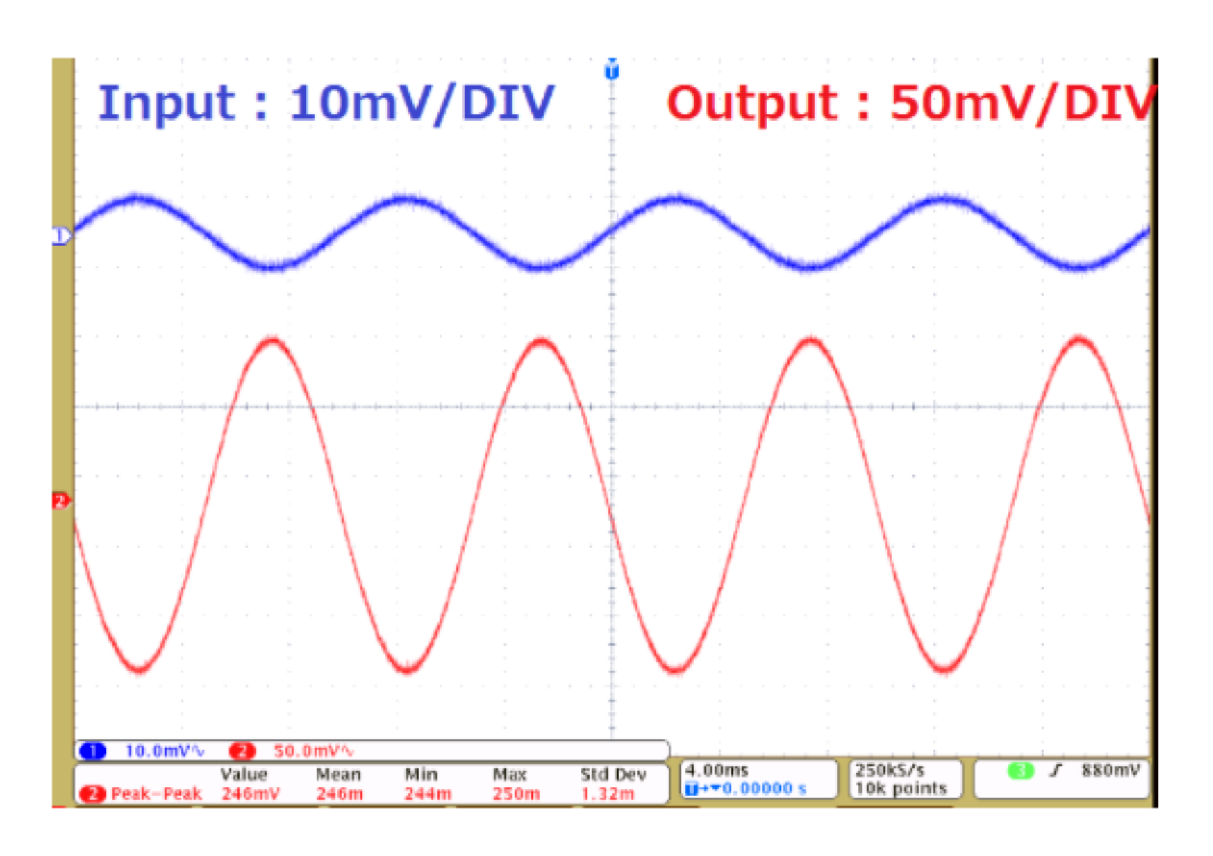
\includegraphics[clip, width=7.0cm]{./Chapter/Chapter3/Picture/SOISTJ2_InOut.eps}
							\hspace{1.6cm} [a] 入出力電圧の関係
						\end{center}
					\end{minipage}
					\begin{minipage}{0.5\hsize}
						\begin{center}
							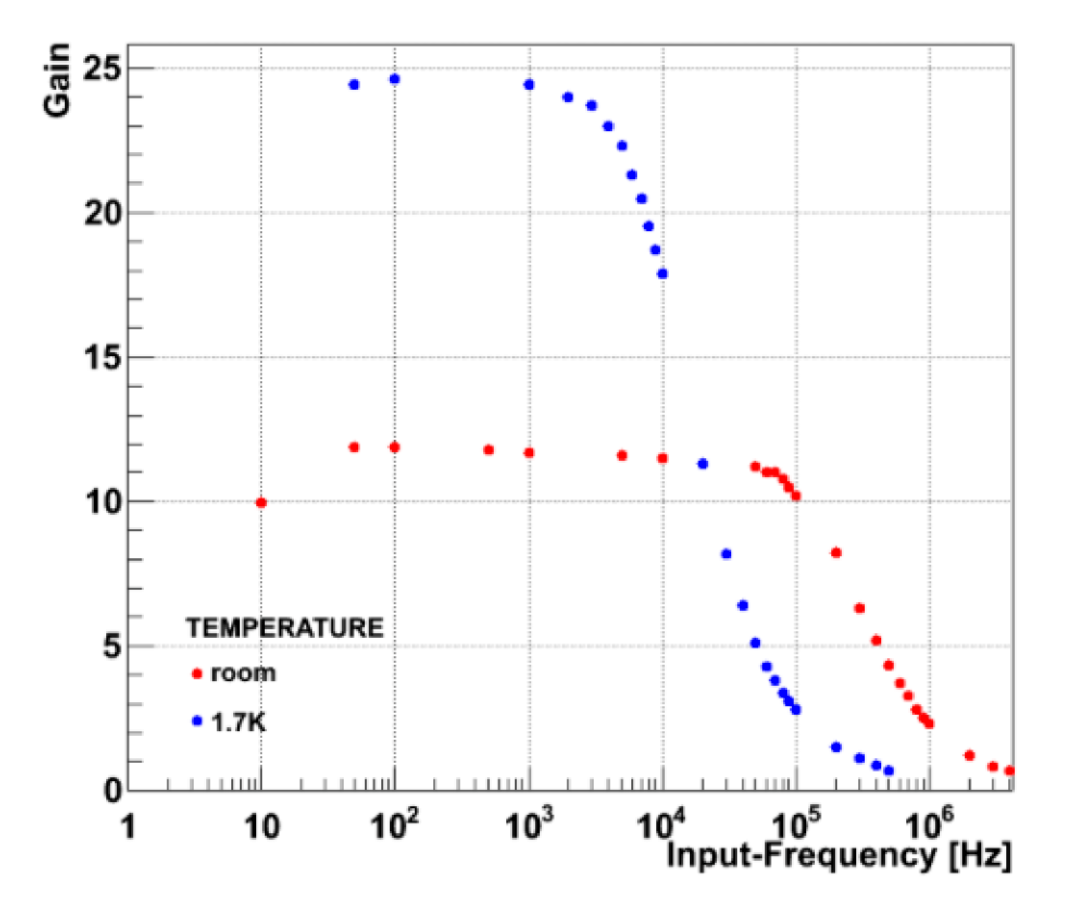
\includegraphics[clip, width=7.0cm]{./Chapter/Chapter3/Picture/SOISTJ2_frequency.eps}
							\hspace{1.6cm} [b] 周波数特性(赤点 : 室温  青点 : 1.7K)
						\end{center}
					\end{minipage}
				\end{tabular}
				\caption{SOI-STJ2の極低温環境下での性能評価}
				\label{fig:SOISTJ2_chara}
			\end{center}
		\end{figure}
		図\ref{fig:SOISTJ2_chara}[a]にSOI-STJ2のソース接地増幅回路における入出力波形を示した。これによると、電圧利得は約25程度獲得できていることが確認できる。
		また図\ref{fig:SOISTJ2_chara}[b]には周波数特性を示した。これによると極低温環境下において入力周波数$1\mathrm{kHz}$程度までは安定して動作していることを確認できる。
		
		これらの結果を踏まえ、SOI-STJ2に新たな問題点が浮上する。
		\begin{description}
			\item[電圧利得が十分ではない]\mbox{}\\
				SOI-STJ2でソース接地増幅回路を組む場合、負荷抵抗を冷凍機配線を介して導入する。
				前述のように電圧利得が十分ではない場合、負荷抵抗を大きくすることでより大きな電圧利得を獲得することができる。
				しかし、それに伴い供給電圧も大きくなり、結果それがMOSFETの耐電圧を超えてしまい素子破壊につながる危険性がある。
			\item[STJ検出器信号速度まで安定して増幅できない]\mbox{}\\
				ソース接地増幅回路のみでは出力インピーダンスが高く、高周波数帯での応答が得られない。
		\end{description}
		
		以上の問題を解決するためにSOI-STJ3の設計が行われた。
		\begin{table}[htb]
			\begin{center}
				\begin{tabular}{| c || c | c | c | c | c |} \hline
					\  & FET Type & Cap. & Channel Width & Channel Length & Gate Cap. \\ \hline \hline
					Pattern1 & Nch & 60pF & $4\mathrm{\mu m} \times 10$ & $1 \mathrm{\mu m}$ & $320 \mathrm{fF}$ \\ \hline
					Pattern2 & Pch & 60pF & $4\mathrm{\mu m} \times 10$ & $1 \mathrm{\mu m}$ & $320 \mathrm{fF}$ \\ \hline
					Pattern3 & Nch & 18pF & $1\mathrm{\mu m} \times 4$ & $1 \mathrm{\mu m}$ & $32 \mathrm{fF}$ \\ \hline
					Pattern4 & Pch & 18pF & $1\mathrm{\mu m} \times 4$ & $1 \mathrm{\mu m}$ & $32 \mathrm{fF}$ \\ \hline
					Pattern5 & Nch & 1.5pF & $1.42\mathrm{\mu m}$ & $0.4 \mathrm{\mu m}$ & $4.5 \mathrm{fF}$ \\ \hline
					Pattern6 & Pch & 1.5pF & $1.42\mathrm{\mu m}$ & $0.4 \mathrm{\mu m}$ & $4.5 \mathrm{fF}$ \\ \hline
				\end{tabular}
				\caption{SOI-STJ2の各パターンごとのFETの詳細}
				\label{tab:SOISTJ2_detail}
			\end{center}
		\end{table}
		\clearpage
	\subsection{3号機(SOISTJ-3)}
		\begin{figure}[htbp]
			\begin{center}
				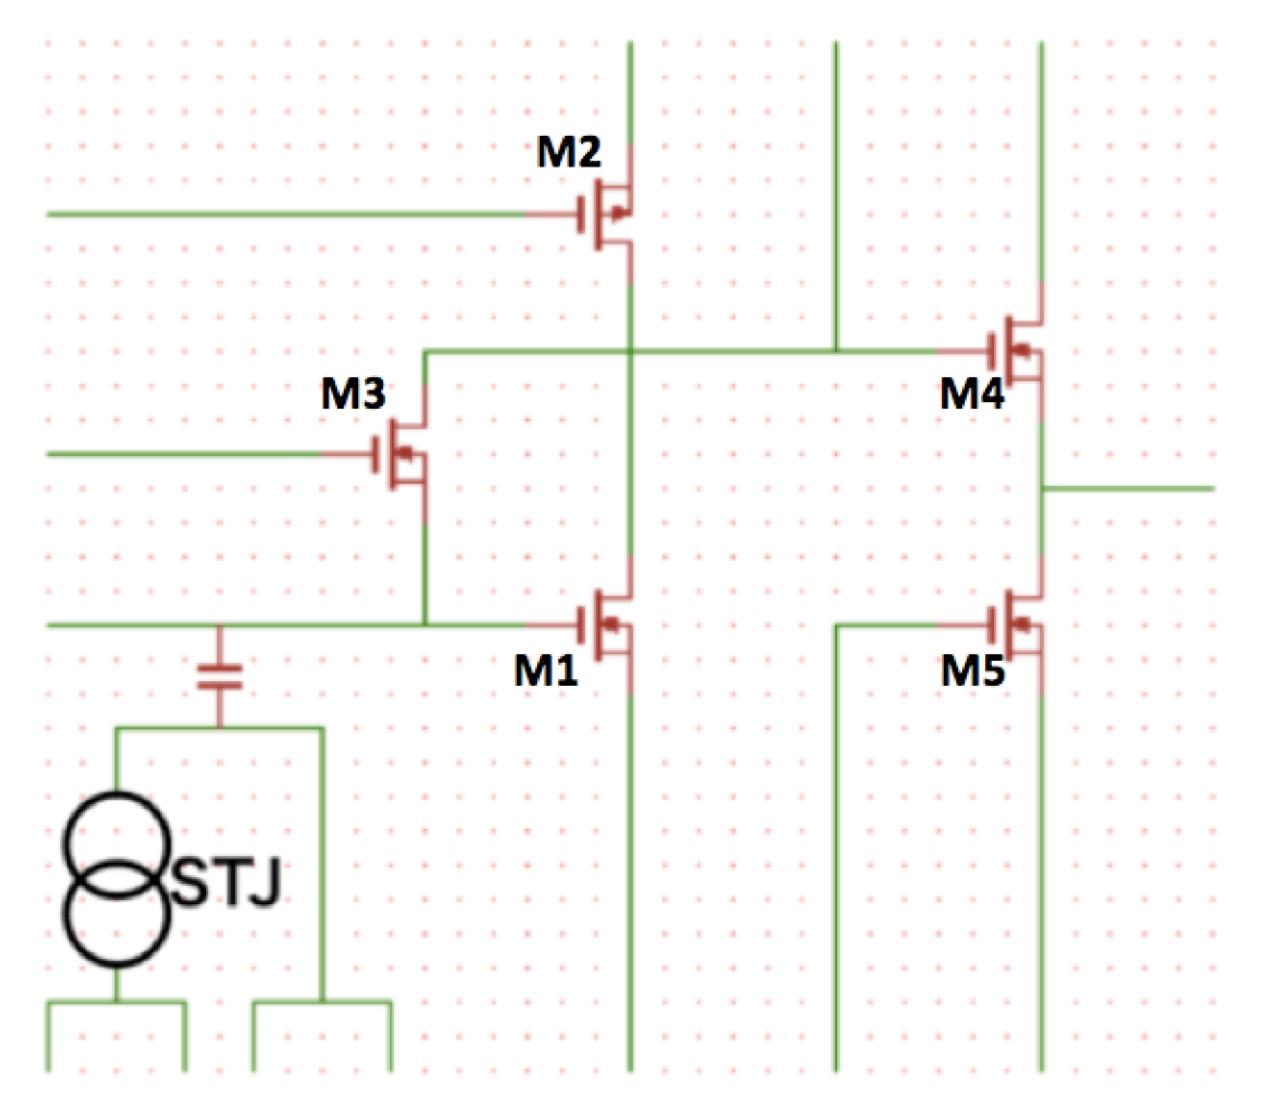
\includegraphics[width=8.0cm]{./Chapter/Chapter3/Picture/SOISTJ3_circuit.eps}
				\caption{極低温環境用SOI前置増幅器3号機(SOI-STJ3)}
				\label{fig:SOISTJ3_circuit}
			\end{center}
		\end{figure}
		\begin{table}[htb]
			\begin{center}
				\begin{tabular}{| c | c | c | c |} \hline
					FET ID & FET Type & Channel Width & Channel Length \\ \hline \hline
					M1 & N\ ch & $2.9 \mathrm{\mu m}$ & $1 \mathrm{\mu m}$ \\ \hline
					M2 & P\ ch & $1 \mathrm{\mu m}$ & $5 \mathrm{\mu m}$ \\ \hline
					M3 & N\ ch & $1 \mathrm{\mu m}$ & $2 \mathrm{\mu m}$ \\ \hline
					M4 & N\ ch & $60 \mathrm{\mu m}$ & $1 \mathrm{\mu m}$ \\ \hline
					M5 & N\ ch & $70 \mathrm{\mu m}$ & $1 \mathrm{\mu m}$ \\ \hline
				\end{tabular}
				\caption{SOI-STJ3に形成されているMOSFETの詳細}
				\label{tab:SOISTJ3_detail}
			\end{center}
		\end{table}
		SOI-STJ2での問題点解決のために、新たにSOI-STJ3を設計した。回路図を図\ref{fig:SOISTJ3_circuit}に示す。
		問題解決のために、以下の変更を行った。
		\begin{enumerate}
			\item NMOS(M3)の導入
			\item PMOS(M2)の導入
			\item ソースフォロアによるバッファ回路(M4とM5)の導入
		\end{enumerate}
		以下、各変更点についての詳細について述べる。
		\begin{description}
			\item[変更点1]\mbox{}\\
				M3を導入することによって、これは増幅段に用いるM1のゲート・ドレイン間の可変抵抗として動作する。
				これによって、M1をソース接地増幅回路として動作させるための適切なゲート電圧とドレイン電圧を設定することができる。
			\item[変更点2]\mbox{}\\
				SOI-STJ2ではソース接地回路としてMOSFETを動作させるために外部から負荷抵抗を導入した。しかし実際には十分な電圧利得を得られていないのが現状である。
				前述の通り負荷抵抗を大きくしすぎると、MOSFETの耐電圧を超える供給電圧が必要になってしまう。
				そこで、負荷抵抗の代わりにMOSFETを電流源負荷として使用するためにM2を導入した。
			\item[変更点3]\mbox{}\\
				SOI-STJ2では出力インピーダンスが非常に大きくなってしまうので、ソースフォロア回路を導入した
		\end{description}
		しかし、今までの増幅器設計の際にSTJ検出器の静電容量を考慮していなかった。
		STJ検出器の静電容量は数十から数百pF程度であるのに対し、SOI-STJ3に形成されたキャパシタンスは数十pF程度である。
		この場合検出器側に比べ増幅回路側のインピーダンスが非常に大きい設計であり、結果図\ref{fig:SOISTJ3_problem}のようにSTJ信号が回路側に伝送されない。\\
		この問題を解決するためにSOI-STJ4の設計を行った。
		\begin{figure}[htbp]
			\begin{center}
				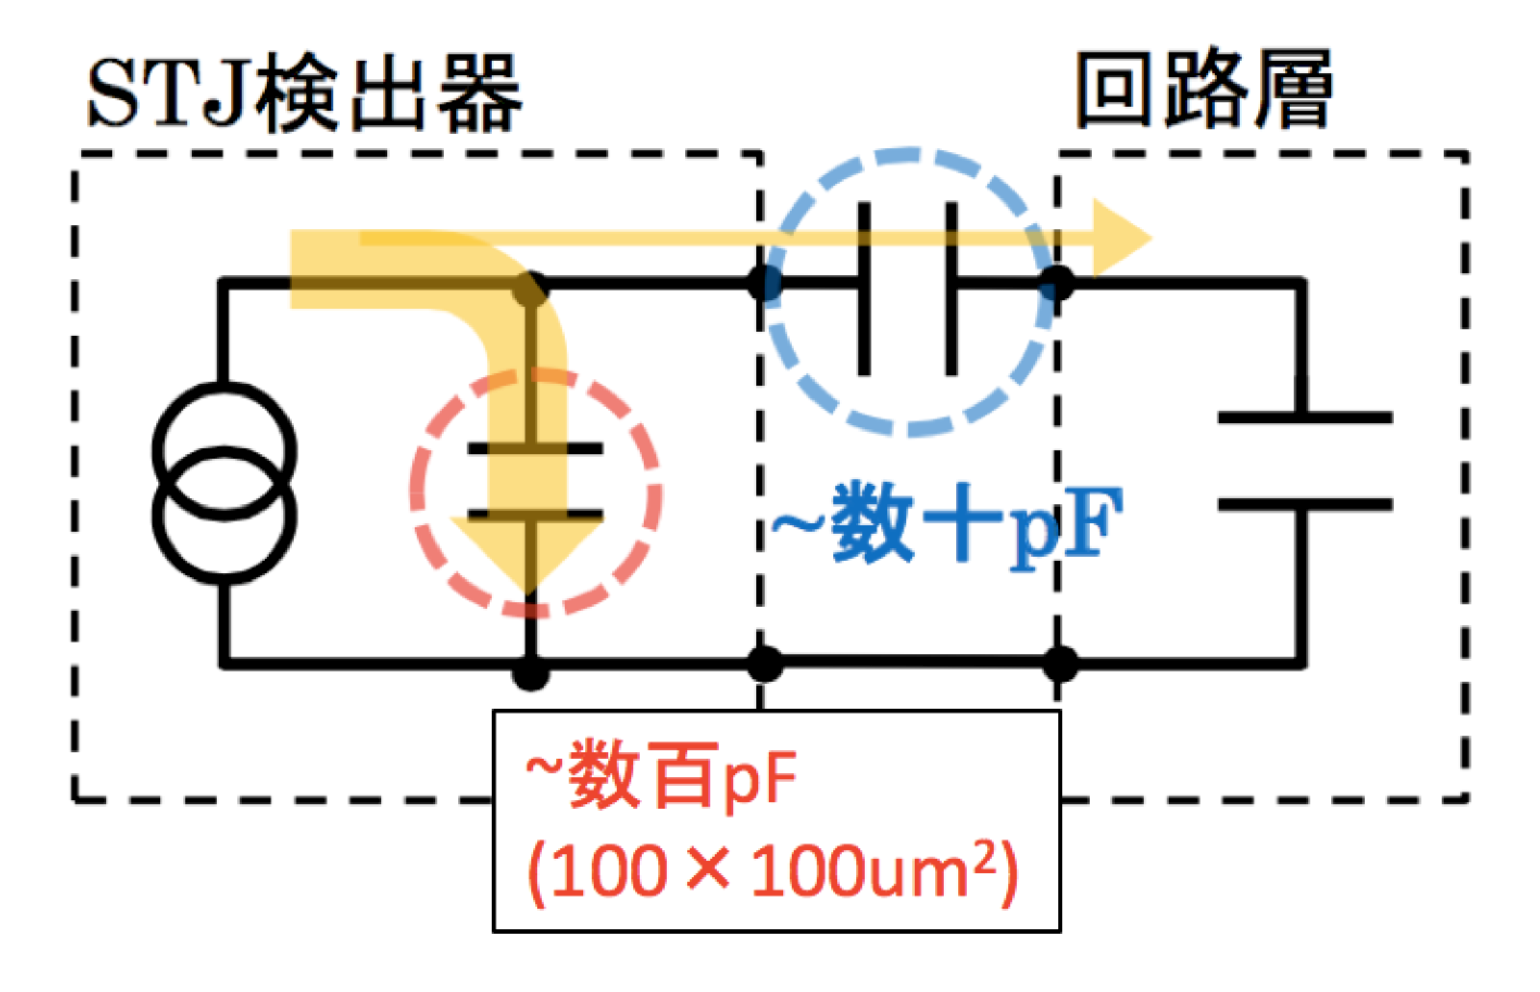
\includegraphics[width=10.0cm]{./Chapter/Chapter3/Picture/SOISTJ3_problem.eps}
				\caption{SOI-STJ3の問題点}
				\label{fig:SOISTJ3_problem}
			\end{center}
		\end{figure}
		\clearpage
	\subsection{4号機(SOI-STJ4)}
		\begin{figure}[htbp]
			\begin{center}
				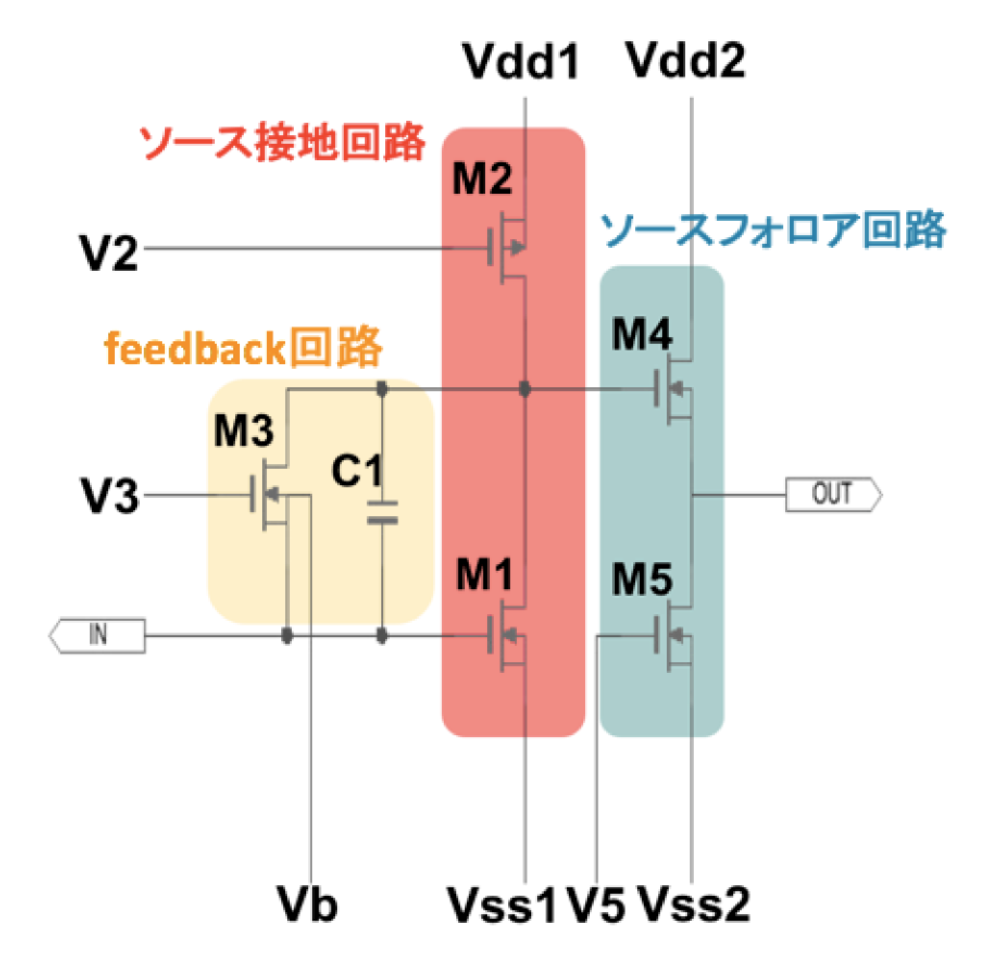
\includegraphics[width=10.0cm]{./Chapter/Chapter3/Picture/SOISTJ4_circuit.eps}
				\caption{極低温環境用SOI前置増幅器4号機(SOI-STJ4)}
				\label{fig:SOISTJ4_circuit}
			\end{center}
		\end{figure}
		\begin{table}[htb]
			\begin{center}
				\begin{tabular}{| c | l | c | c | c |} \hline
					Device ID & Device Type & Channel Width & Channel Length & Cap. \\ \hline \hline
					M1 & core lvt NMOS st2 & $40 \mathrm{\mu m}$ & $1 \mathrm{\mu m}$ & - \\ \hline
					M2 & core lvt PMOS st2 & $1 \mathrm{\mu m}$ & $10 \mathrm{\mu m}$ & - \\ \hline
					M3 & core lvt NMOS bt & $1.6 \mathrm{\mu m}$ & $10 \mathrm{\mu m}$ & - \\ \hline
					M4 & core lvt NMOS st2 & $70 \mathrm{\mu m}$ & $1 \mathrm{\mu m}$ & - \\ \hline
					M5 & core lvt NMOS st2 & $60 \mathrm{\mu m}$ & $1 \mathrm{\mu m}$ & - \\ \hline
					C1 & MIM capacitor & - & - & $100 \mathrm{fF}$ \\ \hline
				\end{tabular}
				\caption{SOI-STJ4に形成されているMOSFETの詳細}
				\label{tab:SOISTJ4_detail}
			\end{center}
		\end{table}
		前述したSOI-STJ3の問題点を解決するために、以下の変更を行った。
		\begin{description}
			\item[フィードバックコンデンサーを加えた]\mbox{}\\
				検出器側から見た入力インピーダンスを下げ、STJ信号を回路側へ伝送しやすくした。
			\item[STJ検出器とSOI-STJ4との間のコンデンサーの除去]\mbox{}\\
				前述の通り、このコンデンサーの静電容量はSTJ検出器の静電容量(数十〜数百pF)よりも十分大きくする必要がある。
				しかし、SOIプロセスで形成できるMIMキャパシタンスは$1.5 \mathrm{fF/{\mu m}^2}$であり、この大容量のキャパシタンスを形成するのは困難である。
				我々はSTJ検出器とSOI-STJ4との間のコンデンサーをSOIプロセスで作製せず、外付けのコンデンサーを用いることにする。
		\end{description}
		そして、SOI-STJ4について極低温環境下での性能評価を行った。
		\begin{figure}[htbp]
			\begin{center}
				\begin{tabular}{c}
					\begin{minipage}{0.5\hsize}
						\begin{center}
							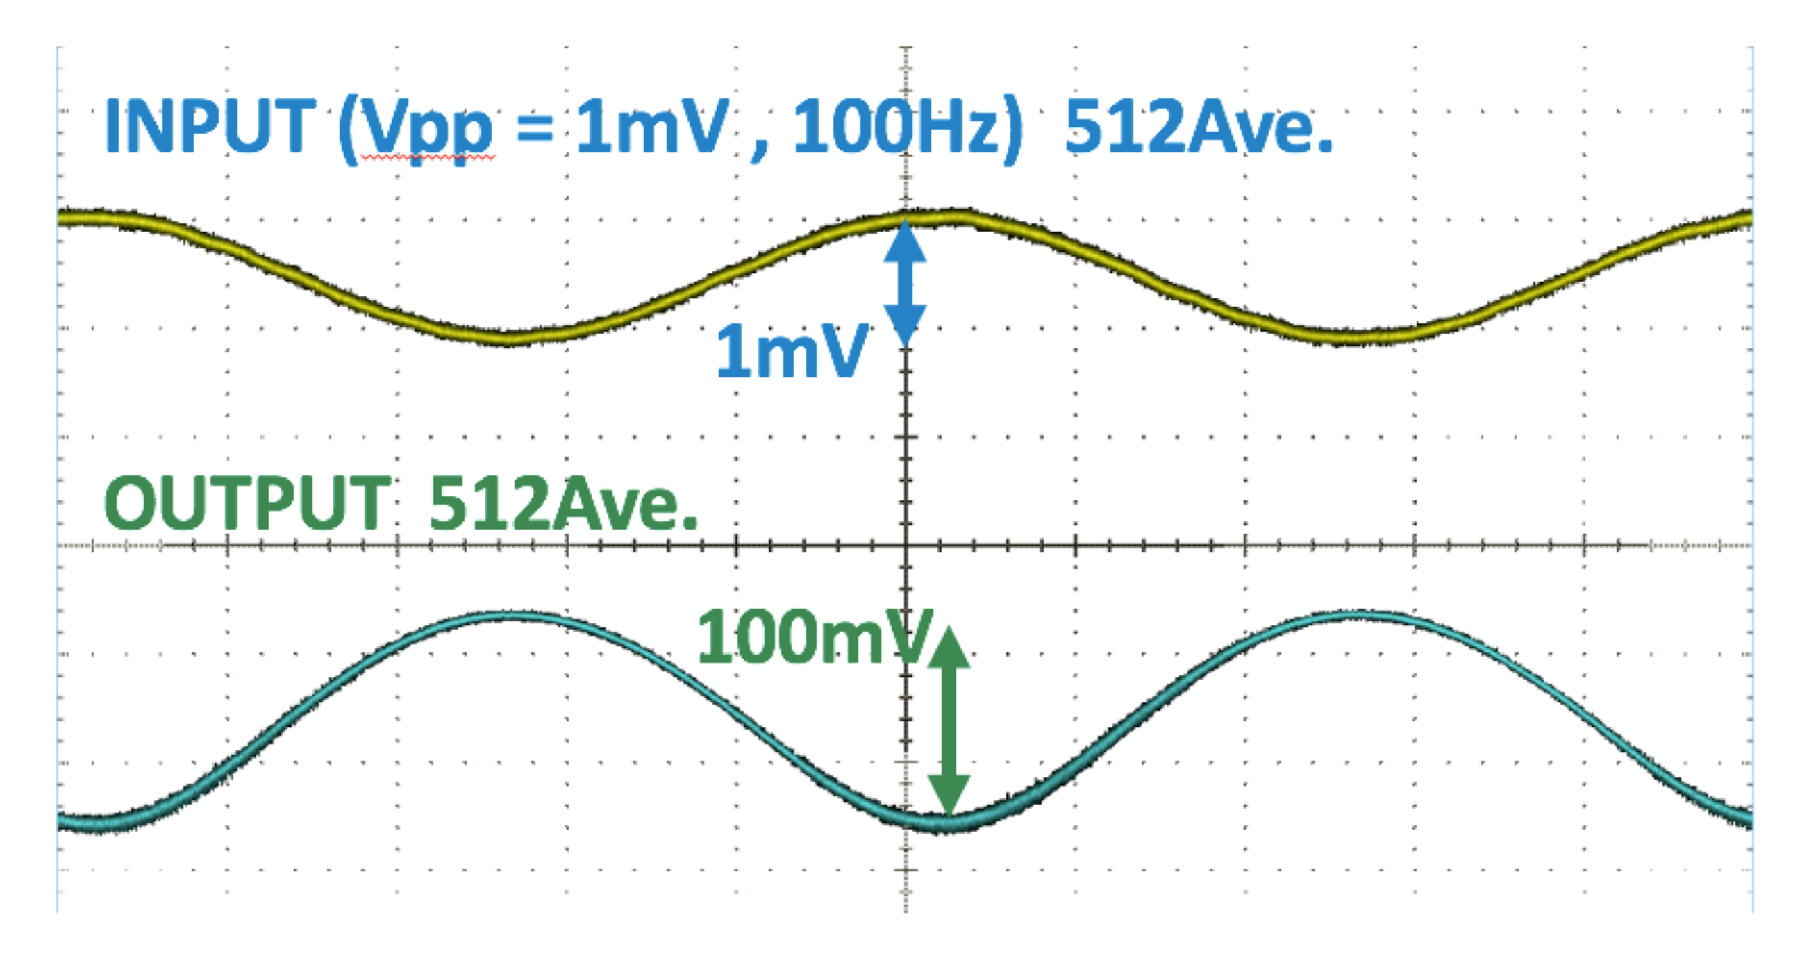
\includegraphics[clip, width=7.0cm]{./Chapter/Chapter3/Picture/SOISTJ4_InOut_100Hz.eps}
							\hspace{1.6cm} [a] 入出力電圧の関係(入力 : sin波(波高 : 1mV  周波数 : 100Hz))
						\end{center}
					\end{minipage}
					\begin{minipage}{0.5\hsize}
						\begin{center}
							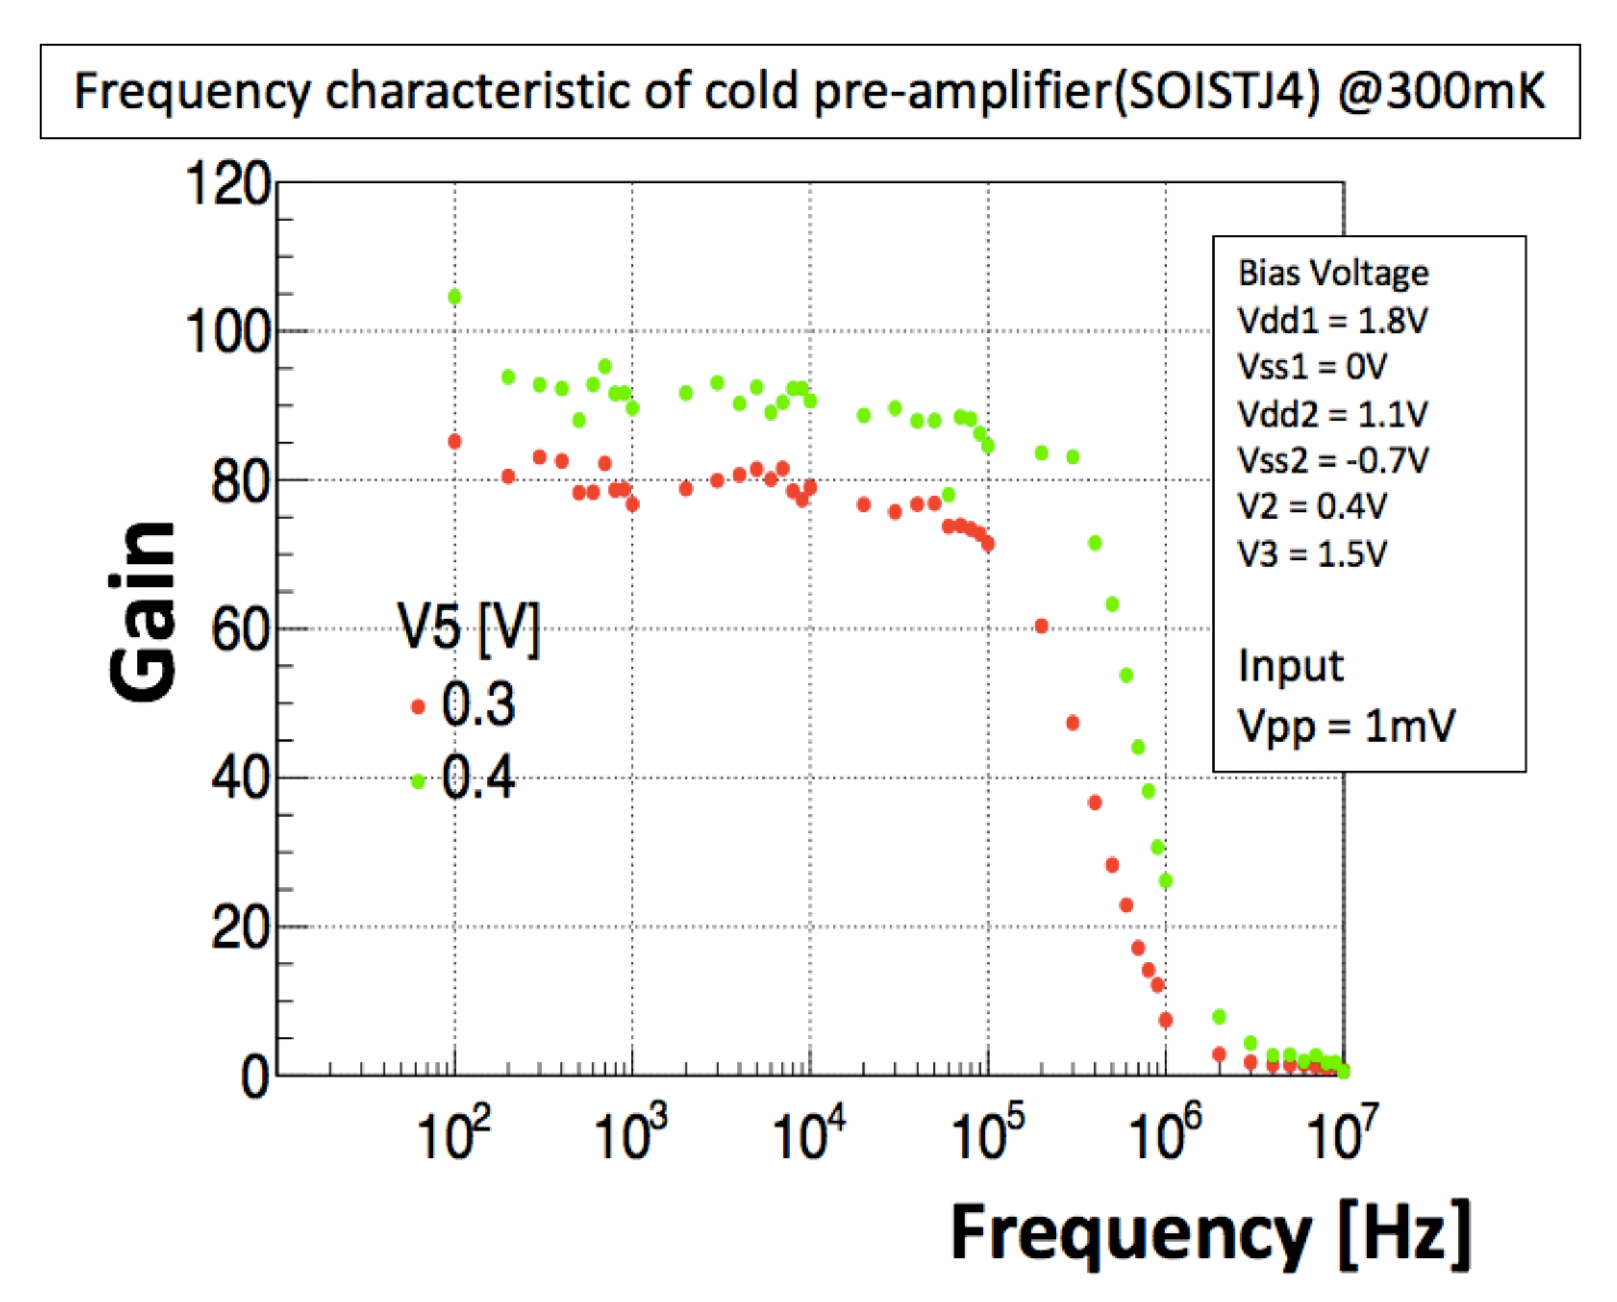
\includegraphics[clip, width=7.0cm]{./Chapter/Chapter3/Picture/SOISTJ4_frequency.eps}
							\hspace{1.6cm} [b] 極低温環境下での周波数特性
						\end{center}
					\end{minipage}
				\end{tabular}
				\caption{SOI-STJ4の極低温環境下での性能評価}
				\label{fig:SOISTJ4_chara}
			\end{center}
		\end{figure}
		\begin{figure}[htbp]
			\begin{center}
				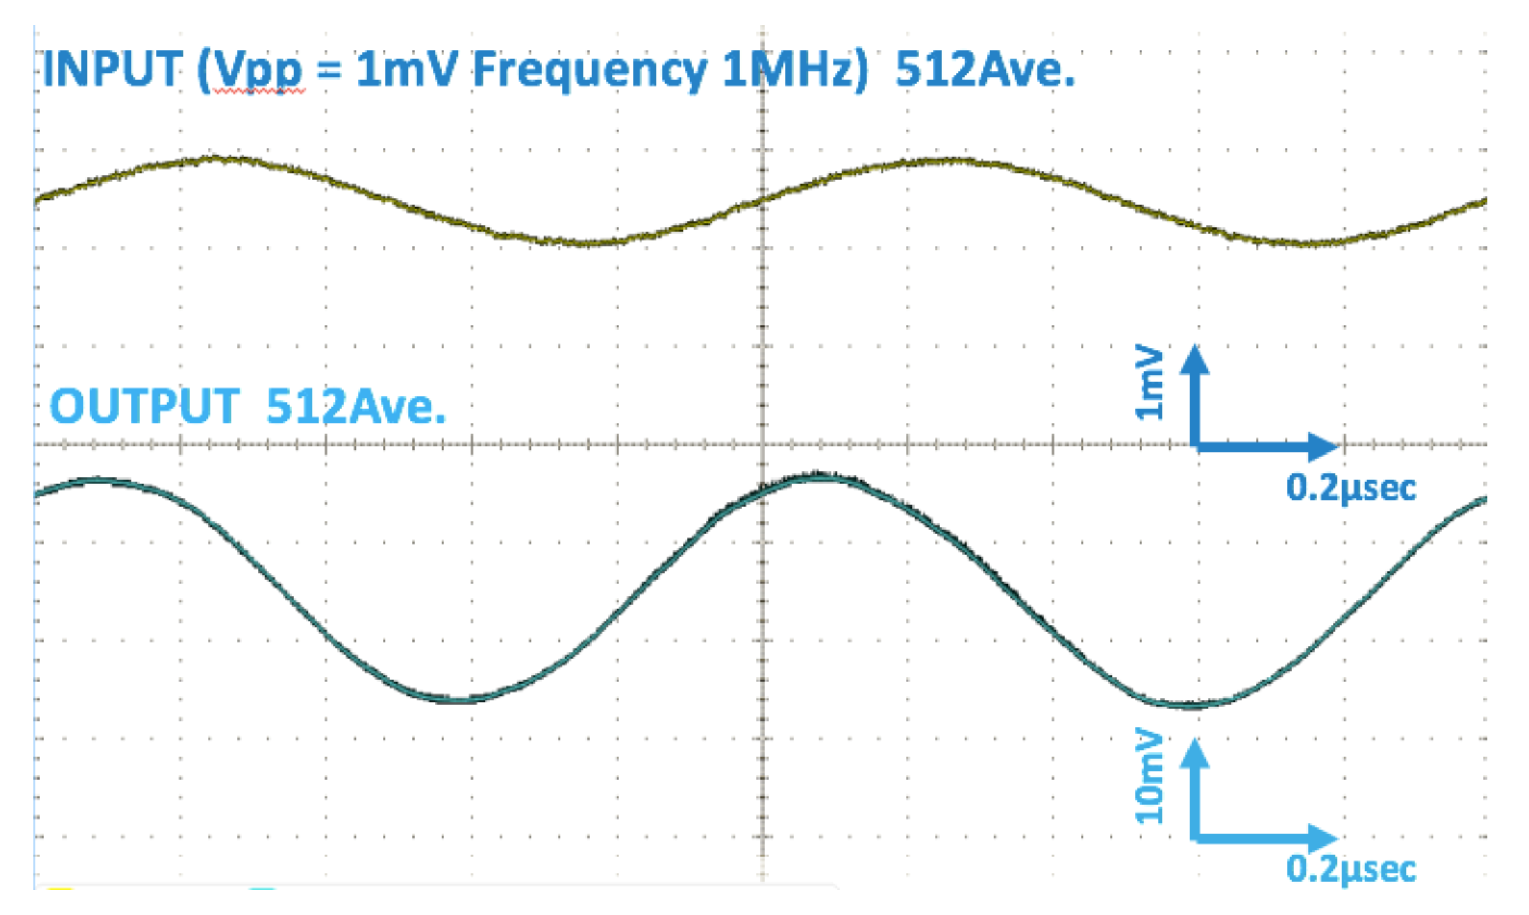
\includegraphics[width=10.0cm]{./Chapter/Chapter3/Picture/SOISTJ4_InOut_1MHz.eps}
				\caption{SOI-STJ4にsin波(波高 : 1mV  周波数 : 1MHz)入力に対する出力}
				\label{fig:SOISTJ4_InOut_1MHz}
			\end{center}
		\end{figure}
		
		図\ref{fig:SOISTJ4_chara}にSOISTJ4の極低温環境下での性能評価を示した。
		図\ref{fig:SOISTJ4_chara}[a]はSOI-STJ4への入出力電圧を示している。黄線はSOI-STJ4への入力sin波(100Hz)であり、青線は出力電圧を示す。
		極低温環境下において、電圧利得は約100程度獲得できていることを確認できた。
		
		また図\ref{fig:SOISTJ4_chara}[b]は極低温環境下での周波数特性を示す。
		これによると、数百kHz程度までは安定して増幅できていることがわかる。
		またSTJ信号速度に対応する1MHzのsin波に対しては電圧利得30〜40を獲得できた。この時の入力と出力の関係を図\ref{fig:SOISTJ4_InOut_1MHz}に示す。
		
		以上より、極低温環境下でもSTJ検出器信号を十分増幅可能な回路が設計されていると考えられる。
		試験的にSTJ検出器に可視光レーザーを照射し、STJ検出器信号をSOI-STJ4に伝送させ増幅させる試験を行った。次章では、その試験結果について報告する。
		
		